%%%%%%%%%%%%%%%%%%%%%%%%%%%%%%%%%%%%%%%%%%%%%%%%%%%%%%%%%%%%%%%%%%%%%%%%%%%%%%%%
%2345678901234567890123456789012345678901234567890123456789012345678901234567890
% 1 2 3 4 5 6 7 8

%%%%%%%%%%%%%%%%%%%%%%%%%%%%%%%%%%%%%%%%%%%%%%%%%%%%%%%%%%%%%%%%%%%%%%%%%%%%%%%%

% \addtolength{\textheight}{-3cm} % This command serves to balance the column lengths
% on the last page of the document manually. It shortens
% the textheight of the last page by a suitable amount.
% This command does not take effect until the next page
% so it should come on the page before the last. Make
% sure that you do not shorten the textheight too much.

%%%%%%%%%%%%%%%%%%%%%%%%%%%%%%%%%%%%%%%%%%%%%%%%%%%%%%%%%%%%%%%%%%%%%%%%%%%%%%%%

\documentclass[conf]{new-aiaa}
%\documentclass[journal]{new-aiaa} % for journal papers
\usepackage[utf8]{inputenc}

\usepackage{graphicx}
\usepackage{amsmath}
\let\Bbbk\relax 
\usepackage{amssymb}
\usepackage{mathtools} % provides \eqqcolon, used in saturation derivation
\usepackage{longtable,tabularx}
\setlength\LTleft{0pt}
\usepackage{booktabs}
\usepackage{multirow}
\usepackage{url}
\usepackage{pdfpages}
\usepackage{float}
\DeclareMathOperator{\s}{s}
\DeclareMathOperator{\cs}{c}
\DeclareMathOperator{\tn}{t}
\DeclareMathOperator{\sat}{sat}
\DeclareMathOperator{\sgn}{sgn}
\allowdisplaybreaks[4]
\emergencystretch=3em

\setcounter{MaxMatrixCols}{15}

% See the \addtolength command later in the file to balance the column lengths
% on the last page of the document

% The following packages can be found on http:\www.ctan.org
%\usepackage{graphics} % for pdf, bitmapped graphics files
%\usepackage{epsfig} % for postscript graphics files
%\usepackage{mathptmx} % assumes new font selection scheme installed
%\usepackage{times} % assumes new font selection scheme installed
%\usepackage{amsmath} % assumes amsmath package installed
%\usepackage{amssymb} % assumes amsmath package installed

\title{Discrete Sliding Mode Control with Actuator Constraints for the Stabilization of a Ballistically Launched Drone}

%\author{ \parbox{3 in}{\centering Huibert Kwakernaak*
% \thanks{Use the $\backslash$thanks command to put information here}\
% Faculty of Electrical Engineering, Mathematics and Computer Science\
% University of Twente\
% 7500 AE Enschede, The Netherlands\
% {\tt\small h.kwakernaak@autsubmit.com}}
% \hspace{ 0.5 in}
% \parbox{3 in}{ \centering Pradeep Misra**
% \thanks{**The footnote marks may be inserted manually}\
% Department of Electrical Engineering \
% Wright State University\
% Dayton, OH 45435, USA\
% {\tt\small pmisra@cs.wright.edu}}
%}

\author{John E. Pye, John-Paul Clarke, and Maruthi Akella%
\footnote{This work was supported by the University of Texas at Austin Cockrell School Fellowship.}%
\footnote{J. E. Pye, JP Clarke, and M. R. Akella are with the Department of Aerospace Engineering, University of Texas at Austin, Austin, TX 78712, USA,
{\tt\small jep4477@my.utexas.edu, johnpaul@utexas.edu, makella@mail.utexas.edu}}}
\affil{Department of Aerospace Engineering, University of Texas at Austin, Austin, TX 78712, USA}

\begin{document}

\maketitle

%%%%%%%%%%%%%%%%%%%%%%%%%%%%%%%%%%%%%%%%%%%%%%%%%%%%%%%%%%%%%%%%%%%%%%%%%%%%%%%%
\begin{abstract}
Highly unstable initial states, such as those produced by ballistic deployment, require nonlinear controllers to stabilize the tumble before the vehicle crashes. We derive and test two nonlinear controllers certified through Lyapunov stability analysis: a continuous-time Sliding Mode controller (cSMC) and a discrete-time Sliding Mode Control (dSMC). We test these against two off-the-shelf controllers: the Linear Quadratic Regulator with Integral Action (LQR) and the cascaded Proportional-Integral-Derivative (PID) controller. We find that the dSMC recovers more of the ballistic-deployment envelope than the LQR, PID, or continuous-time controllers, but that naively clipping the motor speeds to their physical limits---with no intelligent saturation strategy---sharply reduces landing-site reachability. We then extend the dSMC to account for possible motor control constraints in terms of maximum squared rotational speed. If the desired motor speeds fall within the physical bounds, then the augmented controller and the ideal controller are identical, and we satisfy the exponential reaching law. Otherwise, we saturate the control inputs in order of priority (first yaw, then altitude/thrust, then pitch/roll), and obtain weaker input-to-state stability (ISS). However, despite this weaker stability, this priority-weighted saturation increases average landing-site reachability roughly fourfold, from $7.9\%$ (per-motor clipping) to $32.9\%$ (saturation algorithm).
\end{abstract}
%%%%%%%%%%%%%%%%%%%%%%%%%%%%%%%%%%%%%%%%%%%%%%%%%%%%%%%%%%%%%%%%%%%%%%%%%%%%%%%%
\section{Introduction}
In this paper, we develop a controller for UAV stabilization following ballistic deployment. Current work in ballistically launched UAVs, such as the Caltech SQUID \cite{refs:Bouman2019} or the Texas A\&M TLMAV \cite{refs:Denton2025}, focuses on drones that transition into powered flight at a predetermined point in their ballistic trajectory. Current military research efforts, such as the Launched Effects program \cite{refs:Harper2025}, call for a flexible platform that can be deployed anywhere, requires minimal infrastructure, and can carry arbitrary payloads. For example, quick-reaction drones could deliver medical supplies, a role examined in feasibility modeling studies \cite{refs:Starks2024}. Alternatively, launched drones could create a mobile dispersed sensor network, whether for wide-area surveying \cite{refs:Liang2019} or force-protection surveillance \cite{refs:Michelena2025}. These applications require drones capable of deploying into powered flight at any point along their trajectory. We evaluate the controllers on these test cases by how much of the ballistic-deployment envelope each recovers.

\subsection{Related Work}
The dSMC approach for quadrotor control has been the subject of some limited existing studies. Xiong et. al. \cite{refs:Xiong2016} introduced the unconstrained formulation of the dSMC and presented how a discrete Lyapunov stability condition may be satisfied for arbitrary discretization sampling times. Xu et al. \cite{refs:Xu2020} introduced per-channel auxiliary states for the three attitude moments of a quadrotor using SMC under input saturation, and proved closed-loop stability via Lyapunov analysis. Kuang and Chen \cite{refs:Kuang2024} adopted a vector-valued second-order auxiliary controller for the position and attitude loops together with a disturbance observer and adaptive laws for unknown mass and inertia. Shao et al.\ \cite{refs:Shao2022}, on the other hand, embedded a bounded saturation function directly in the control law alongside adaptive parameters. However, these works are all in the continuous time space, and do not cover the collective-thrust control channel together with the three torque channels in a single per-motor construction. 

While these saturation methods do not incorporate control prioritization, Faessler et al.\ \cite{refs:Faessler2017} present an explicit prioritization of roll and pitch torques above collective thrust above yaw torque under motor saturation, and build the priority into an iterative mixer without formal stability assurances. Similarly, Mueller and D’Andrea \cite{refs:Mueller2013} linearize their input constraints inside an MPC loop. We use the same priority order ($M_x, M_y \succ T \succ M_z$) but solve the projection over the squared rotor speed $\Omega^2$-space and carry it through to the closed-loop stability proof.

In addition to retaining the basic Lyapunov stability bounds, Wang et al.\ \cite{refs:Wang2005} give us the discrete-time component-wise saturation model and the saturation-dependent Lyapunov approach we extend to characterize the admissible control space $\mathcal{U}$, and Jiang and Wang \cite{refs:JiangWang2001} provide the discrete-time input-to-state-stability (ISS) Lyapunov framework we use to demonstrate the ISS form of our closed-loop result. The discrete reaching-law boundary $\eta\,\Delta t < 2$, which follows from the discrete-time sliding-mode existence condition $|s_{k+1}| < |s_k|$ of Sarpturk et al.\ \cite{refs:Sarpturk1987}, drops out as a special case when the deficit $\Delta u_k$ vanishes; the unconstrained dSMC structure follows the discrete-time formulation of Xiong and Zhang \cite{refs:Xiong2016}.

\subsection{New Contributions}
We present a corrected derivation with formal Lyapunov stability analysis of the Discrete Sliding Mode Controller (dSMC) presented in \cite{refs:Xiong2016}. We also extend the dSMC to include per-motor speed limits, which equate to control effort saturation in collective thrust, and roll, pitch, and yaw moments. We compare this to a reformulated Continuous Sliding Mode Controller (cSMC), similar to the form derived in \cite{refs:Tahir2020}. We compare these two SMC formulations against classical LQR and cascaded PID, both of which are common commercial off-the-shelf (COTS) drone control solutions. Our dSMC corrects and re-derives the control laws in \cite{refs:Xiong2016}, whose proposed forms violate the exponential reaching condition and produce an unstable or unresponsive controller. We also introduce a new test case, the stabilization of a ballistically launched quadrotor into powered flight, which suggests that the results of \cite{refs:Tahir2020} hold only for a limited range of initial conditions. Lastly, we reformulate the dSMC controller with control saturation. We first apply control-priority weighting (with pitch and roll weighted as more important than total thrust, which in turn is weighted as more important than yaw). Then, we augment each control channel with auxiliary states and, once again, apply the exponential reaching law analysis, demonstrating that the reaching laws hold under transient control saturation. When commands are naturally feasible, we recover the unconstrained dSMC controller. In the presence of control saturation, we demonstrate an input-to-state stability bound (provided the saturation is not permanent). This approach is similar to \cite{refs:Wang2005, refs:JiangWang2001}, but we adapt these methods to discrete time control with a separate scalar auxiliary state per actuator channel (including total thrust) and show that we still maintain the Lyapunov bound of the underlying dSMC under transient saturation. We also examine a new application of the controller; ballistic transition stabilization and landing.

\begin{table}[!htbp]
\centering
\caption{Nomenclature and Variables}
\label{tab:constants}
\renewcommand{\arraystretch}{0.90}
\begin{tabular}{lll}
\toprule
\textbf{Symbol} & \textbf{Description} & \textbf{Value} \\
\midrule
\multicolumn{3}{l}{\textbf{Model parameters}} \\
$k_{MT}$ & Ratio of motor torque to thrust & $0.1\,\text{m}$ \\
$l$ & Quadrotor arm length & $0.2\,\text{m}$ \\
$J_{xx}$ & Moment of inertia about body $x$ axis & $1.8\times10^{-3}\,\text{kg}\cdot\text{m}^2$ \\
$J_{yy}$ & Moment of inertia about body $y$ axis & $1.8\times10^{-3}\,\text{kg}\cdot\text{m}^2$ \\
$J_{zz}$ & Moment of inertia about body $z$ axis & $1.5\times10^{-3}\,\text{kg}\cdot\text{m}^2$ \\
$m$ & Drone mass & $0.8\,\text{kg}$ \\
$g$ & Acceleration due to gravity & $9.81\,\text{m/s}^2$ \\
$J_r$ & Rotor moment of inertia about the spin axis of the motor & $\approx 0$ \\
$\kappa$ & Gyroscopic coupling between rotors and body & $\approx 0$ (see text) \\
\midrule
\multicolumn{3}{l}{\textbf{State variables}} \\
$v_x, v_y, v_z$ & Body-frame velocity components & -- \\
$\omega_x, \omega_y, \omega_z$ & Body-frame rotation rates & -- \\
$\theta, \phi, \psi$ & Pitch, roll, and yaw Euler angles (Z-Y-X order) & -- \\
$x, y, z$ & Inertial position; north, east positive; $z$ upward (altitude) & -- \\
\midrule
\multicolumn{3}{l}{\textbf{Motor mixing}} \\
$T$ & Net thrust along the body $z$ axis & -- \\
$M_x, M_y, M_z$ & Moments about the body $x$, $y$, $z$ axes & -- \\
$T_i$ & Thrust produced by rotor $i$, $i \in \{1,\dots,4\}$ & -- \\
$\omega_i$ & Angular velocity of rotor $i$ & -- \\
$\Omega_i^2$ & Squared angular velocity of rotor $i$ & -- \\
$\Omega_r$ & Net rotor speed differential $\omega_1-\omega_2+\omega_3-\omega_4$ & -- \\
$\Omega^2_{\min}, \Omega^2_{\max}$ & Per-rotor squared-speed bounds & $0,\ 2$ (normalized) \\
$T_M$ & Mixing matrix from $\Omega^2$ to $(T, M_x, M_y, M_z)^T$ & -- \\
$b$ & Per-rotor thrust per squared rotor speed & $5$ (normalized) \\
$d$ & Per-rotor yaw torque per squared rotor speed & $2$ (normalized) \\
$u_k$ & Commanded control at step $k$, $(T, M_x, M_y, M_z)^T$ & -- \\
$\bar u_k$ & Saturated command after projection onto $\mathcal{U}$ & -- \\
$\Delta u_k$ & Saturation deficit, $u_k - \bar u_k$ & -- \\
$\mathcal{U}$ & Feasible control set under per-rotor speed limits & -- \\
\midrule
\multicolumn{3}{l}{\textbf{Sliding mode control and saturation}} \\
$s_\alpha$ & Sliding surface for channel $\alpha \in \{T, M_x, M_y, M_z\}$ & -- \\
$\tilde s_k$ & Modified sliding surface, $s_k - D_k\,\xi_k$ & -- \\
$e_\alpha$ & Tracking error for channel $\alpha$ & -- \\
$\eta_\alpha$ & Reaching-law gain for channel $\alpha$ & -- \\
$\xi_k$ & Per-channel auxiliary state vector & -- \\
$k_{\xi,\alpha}$ & Contraction rate of the auxiliary-state filter & -- \\
$D_k$ & Coupling between the auxiliary state and the sliding surface & -- \\
$V_k$ & Discrete Lyapunov function at step $k$ & -- \\
\midrule
\multicolumn{3}{l}{\textbf{Model discretization}} \\
$\Delta t$ & Discrete control sample interval & $0.02\,\text{s}$ \\
$k$ & Discrete-time index & -- \\
\bottomrule
\end{tabular}
\end{table}
\begin{figure}[H]
\centering
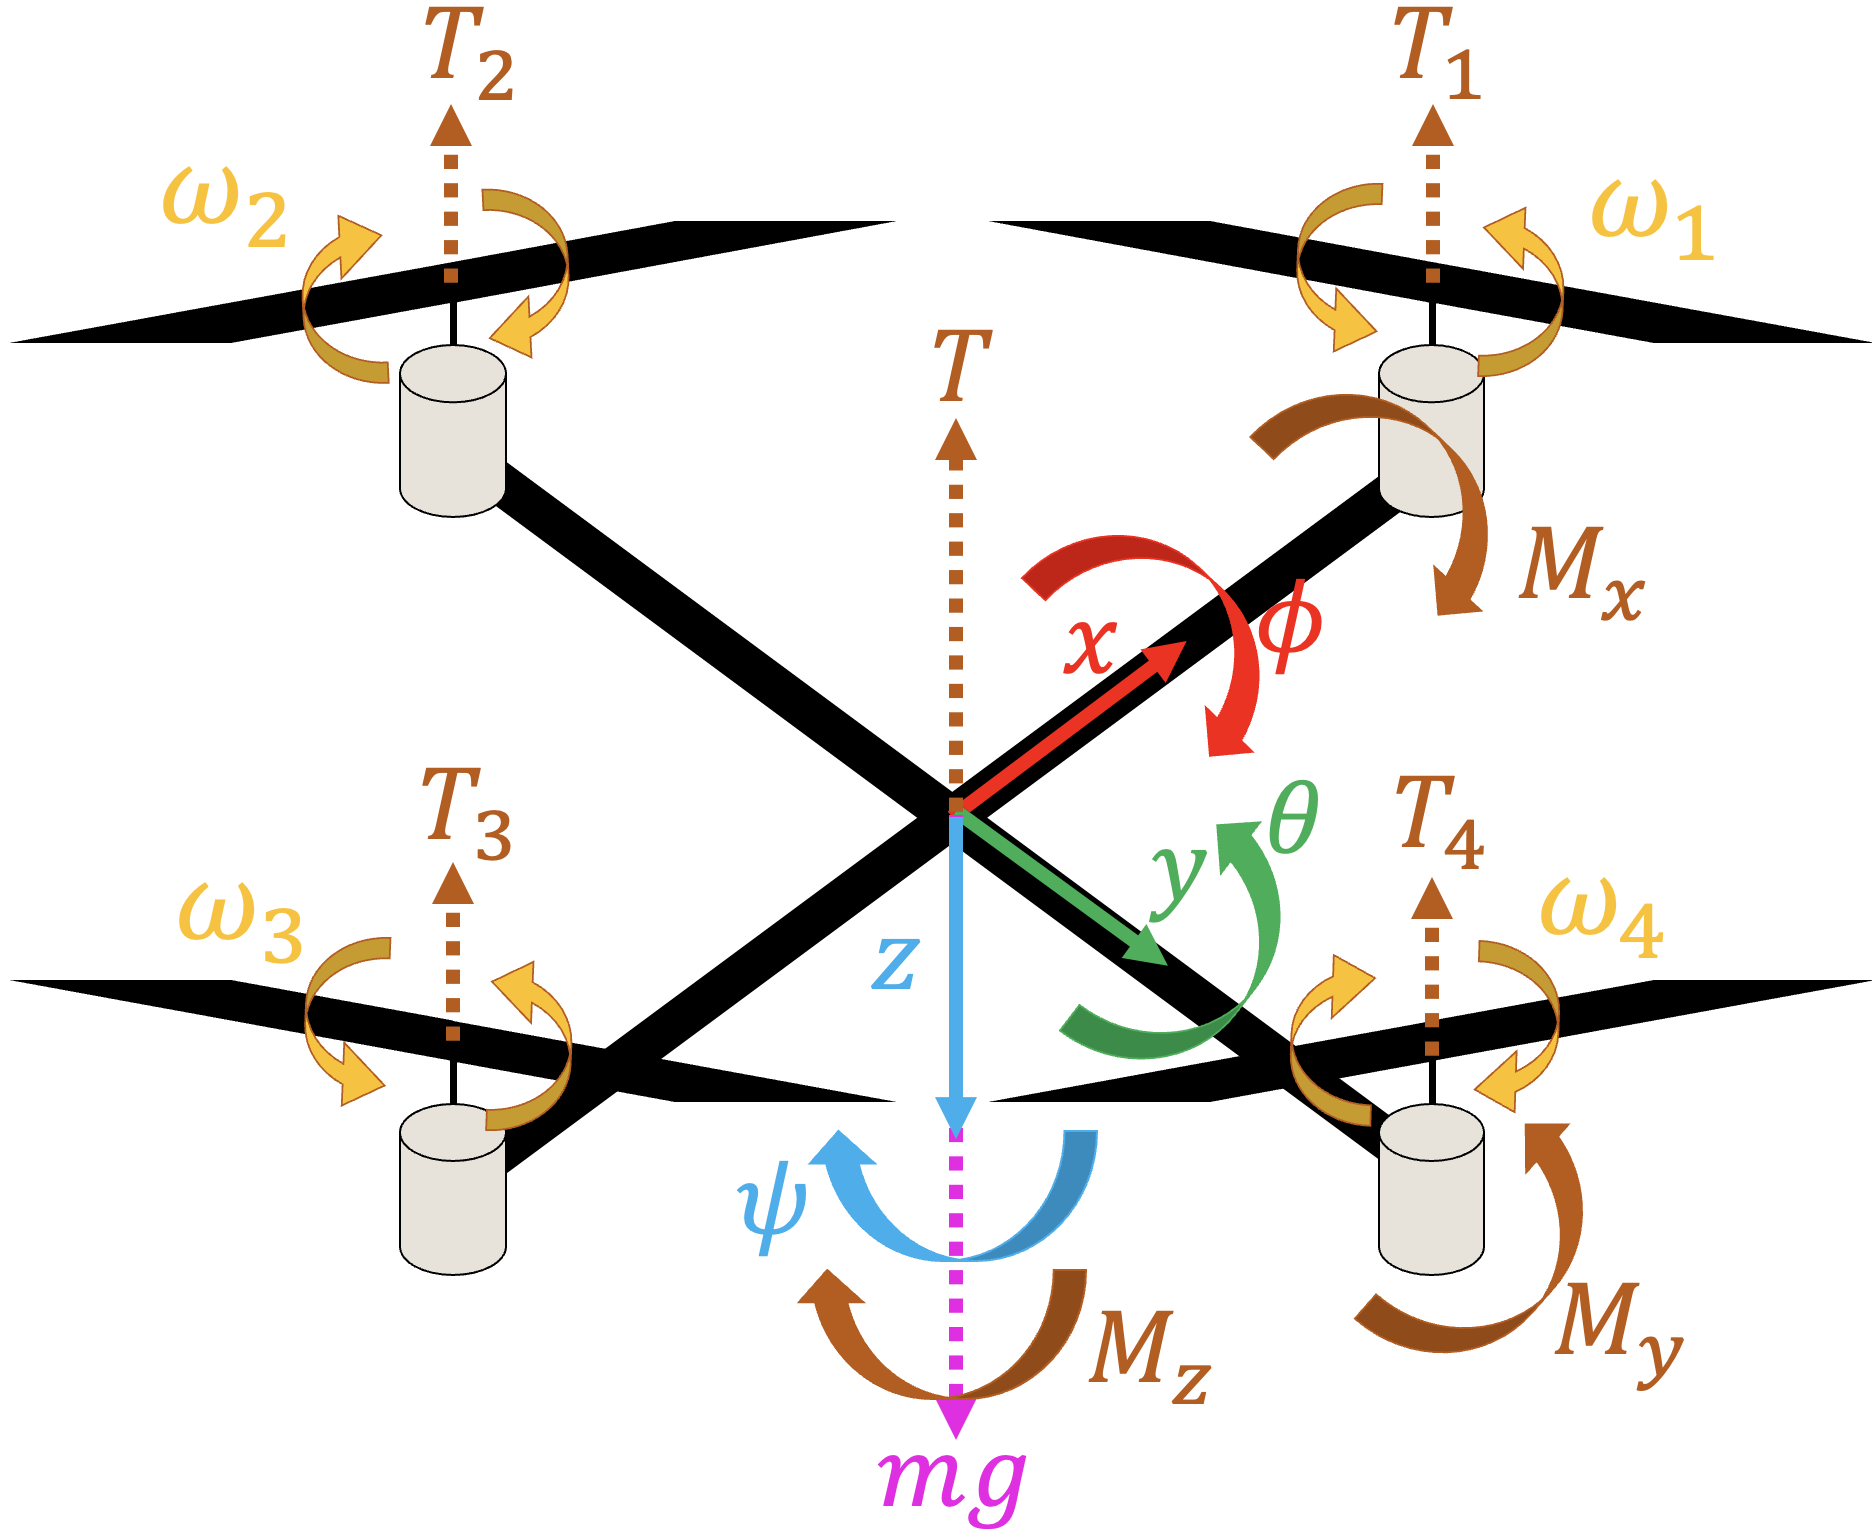
\includegraphics[width=0.5\linewidth]{figs/quadrotor.png}
\caption{Quadrotor coordinate system and force vectors.}
\label{fig:quadrotor}
\end{figure}
\section{Vehicle Model}
We apply the controllers derived in this paper to the standard symmetric quadrotor in a North-East-Down inertial coordinate frame with Z-Y-X Euler angle rotation order. We use the standard nonlinear and linear system of equations presented in \cite{refs:Tahir2020}. The model parameters are given in Table \ref{tab:constants}. We choose to work in the force-moment space ($T$ for net thrust along the body $z$ axis and $M_x, M_y, M_z$ for the moments about the body $x$, $y$, and $z$ axes), rather than the individual rotor angular velocities ($\omega_1, \omega_2, \omega_3, \omega_4$), without loss of generality due to the linear mapping from squared rotor velocities to force-moments.

\begin{equation}
\label{eq:thrusts}
\begin{bmatrix}
T \\ M_x \\ M_y \\ M_z
\end{bmatrix}
=
\begin{bmatrix}
1 & 1 & 1 & 1 \\
0 & -l & 0 & l \\
-l & 0 & l & 0 \\
k_{MT} & -k_{MT} & k_{MT} & -k_{MT}
\end{bmatrix}
\begin{bmatrix}
T_1 \\ T_2 \\ T_3 \\ T_4
\end{bmatrix}.
\end{equation}

The full nonlinear system of equations of motion is given in Equation \ref{eq:nonlinear-eom}, where $v_x, v_y, v_z$ are the body-frame velocity components, $\omega_x, \omega_y, \omega_z$ are the body-frame attitude rates, $\theta, \phi, \psi$ are the inertial pitch, roll, and yaw Euler angles, and $x, y, z$ are the inertial position (north and east positive; the $z$ position is expressed as altitude, positive upward).

\small
\begin{equation}
\label{eq:nonlinear-eom}
\setlength{\arraycolsep}{3pt}
\begin{array}{rclcrclcrcl}
\dot v_x &=& -v_z\,\omega_y + v_y\,\omega_z - g\,\s\theta, &\quad&
\dot v_y &=& -v_x\,\omega_z + v_z\,\omega_x + g\,\cs\theta\,\s\phi, &\quad&
\dot v_z &=& -v_y\,\omega_x + v_x\,\omega_y + g\,\cs\theta\,\cs\phi - \tfrac{T}{m}, \\[3pt]
\dot\omega_x &=& \begin{aligned}[t]
&\tfrac{1}{J_{xx}}\bigl[\,{-}\omega_y\,\omega_z(J_{zz}{-}J_{yy}) \\
&\quad + M_x - \kappa\,M_z\,\omega_y\bigr],
\end{aligned} &&
\dot\omega_y &=& \begin{aligned}[t]
&\tfrac{1}{J_{yy}}\bigl[\,{-}\omega_x\,\omega_z(J_{xx}{-}J_{zz}) \\
&\quad + M_y - \kappa\,M_z\,\omega_x\bigr],
\end{aligned} &&
\dot\omega_z &=& \tfrac{M_z}{J_{zz}}, \\[3pt]
\dot\theta &=& \omega_y\,\cs\phi - \omega_z\,\s\phi, &&
\dot\phi &=& \omega_x + \omega_y\,\s\phi\,\tn\theta + \omega_z\,\cs\phi\,\tn\theta, &&
\dot\psi &=& \tfrac{\omega_y\,\s\phi + \omega_z\,\cs\phi}{\cs\theta}, \\[3pt]
\dot x &=& \begin{aligned}[t]
&v_x\,\cs\psi\,\cs\theta \\
&+ v_y(-\s\psi\,\cs\phi + \cs\psi\,\s\theta\,\s\phi) \\
&+ v_z(\s\psi\,\s\phi + \cs\psi\,\s\theta\,\cs\phi),
\end{aligned} &&
\dot y &=& \begin{aligned}[t]
&v_x\,\s\psi\,\cs\theta \\
&+ v_y(\cs\psi\,\cs\phi + \s\psi\,\s\theta\,\s\phi) \\
&+ v_z(-\cs\psi\,\s\phi + \s\psi\,\s\theta\,\cs\phi),
\end{aligned} &&
\dot z &=& v_x\,\s\theta - v_y\,\cs\theta\,\s\phi - v_z\,\cs\theta\,\cs\phi.
\end{array}
\end{equation}
\normalsize

In the simulations reported here the rotor--body gyroscopic terms are inactive: the rotor spin inertia is negligible ($J_r \approx 0$), and the $\kappa\,M_z\,\omega_x$, $\kappa\,M_z\,\omega_y$ coupling terms are disabled accordingly ($\kappa \to 0$); both are retained in the equations above for generality.

Linearizing the system about the steady-state point (level and stationary) yields a simplified set of equations that we use to derive our LQR controller gains.

\small
\begin{equation}
\label{eq:linear-eom}
\setlength{\arraycolsep}{3pt}
\begin{array}{rclcrclcrcl}
\dot v_x &=& -g\,\theta, &\quad& \dot v_y &=& g\,\phi, &\quad& \dot v_z &=& -T/m, \\[3pt]
\dot\omega_x &=& M_x/J_{xx}, && \dot\omega_y &=& M_y/J_{yy}, && \dot\omega_z &=& M_z/J_{zz}, \\[3pt]
\dot\theta &=& \omega_y, && \dot\phi &=& \omega_x, && \dot\psi &=& \omega_z, \\[3pt]
\dot x &=& v_x, && \dot y &=& v_y, && \dot z &=& -v_z.
\end{array}
\end{equation}
\normalsize

We skip the controllability and observability analysis. The quadrotor is well known to be fully (directly or indirectly) controllable in the nonlinear form above. We assume the full state is observable; on our hardware target, GPS, an onboard IMU, and an EKF provide position, attitude, and translational and rotational velocities with sufficient precision.

%%%%%%%%%%%%%%%%%%%%%%%%%%%%%%%%%%%%%%%%%%%%%%%%%%%%%%%%%%%%%%%%%%%%%%%%%%%%%%%%
\section{Controller Formulation}

\subsection{LQR Controller with Integral Action}
LQR computes a constant state-feedback gain that minimizes an infinite-horizon quadratic cost. The cost function we minimize, given in Equation \ref{eq:lqr}, is the standard form of the LQR cost function with integral action.

\small
\begin{equation}
\label{eq:lqr}
\begin{aligned}
J(u) &= \int_{0}^{\infty} \Bigl( \tilde{x}^{\top} Q\, \tilde{x}
+ u^{\top} R\, u \Bigr)\,\mathrm{d}t \\
\tilde{x} &=
\begin{bmatrix}
\left(\displaystyle \int_{0}^{t} e(\tau)\,\mathrm{d}\tau\right)^{\top} & x^{\top}
\end{bmatrix}^{\top} \\
e &= r - [x, y, z]^{\top},
\qquad
u = \frac{K_i}{s}\, e - K_p\, x
\end{aligned}
\end{equation}
\normalsize

To realize a LQR controller with integral action, we augment our base state vector with three additional states, representing integrated Earth-frame position. This way, we can derive integral gains in addition to proportional gains when we solve the Discrete Algebraic Riccati Equation. We use the following state-cost matrix $Q$ and control-cost matrix $R$, which are the result of manual tuning of the weights presented in \cite{refs:Tahir2020}:
\small
\begin{equation}
\begin{aligned}
Q &= \operatorname{diag}(q) \big/ \bigl|q\bigr|_2, \quad R = I_4, \\
q &= [3,\,3,\,6000,\,1080,\,1080,\,1080,\,180,\,180,\,180,\,0.5,\,0.5,\,1000,\,15,\,15,\,300]^{\top}.
\end{aligned}
\end{equation}
\normalsize

Solving for the optimal proportional and integral gains, we obtain:
{\small
\begin{equation}
\label{eq:lqr-gains}
\begingroup
\setlength{\arraycolsep}{0.5pt}%
\renewcommand{\arraystretch}{1.05}%
\begin{aligned}
K_i &=
\begin{bmatrix}
0 & 0 & 0.22 \\
0 & 0.05 & 0 \\
-0.05 & 0 & 0 \\
0 & 0 & 0
\end{bmatrix}
\\[4pt]
K_p &=
\begin{bmatrix}
0 & 0 & -1.55 & 0 & 0 & 0 & 0 & 0 & 0 & 0 & 0 & 0.91 \\
0 & 0.16 & 0 & 0.42 & 0 & 0 & 0 & 1.56 & 0 & 0 & 0.13 & 0 \\
-0.16 & 0 & 0 & 0 & 0.42 & 0 & 1.16 & 0 & 0 & -0.13 & 0 & 0 \\
0 & 0 & 0 & 0 & 0 & 0.41 & 0 & 0 & 0.17 & 0 & 0 & 0
\end{bmatrix}
\end{aligned}
\endgroup
\end{equation}
}

\subsection{Cascaded PID Controller}
We formulate the standard four-loop cascaded PID controller, with outer and inner loops for both position and attitude. The gains used are given in Table \ref{tab:pid-gains}.

\small
\begin{table}[t]
\centering
\vspace*{8pt}
\caption{PID gains for outer/inner position and attitude loops.}
\label{tab:pid-gains}
\footnotesize
\setlength{\tabcolsep}{4pt}
\renewcommand{\arraystretch}{0.85}
\begin{tabular}{llcccc}
\toprule
\textbf{Loop} & \textbf{Channel} & \textbf{P} & \textbf{I} & \textbf{D} & \textbf{N} \\
\midrule
\multirow{3}{*}{\shortstack[l]{Outer\\positional}}
& $x \to \dot{x}$ & 0.25 & 0 & 0 & – \\
& $y \to \dot{y}$ & 0.25 & 0 & 0 & – \\
& $z \to \dot{z}$ & 0.40 & 0 & 0 & – \\
\midrule
\multirow{3}{*}{\shortstack[l]{Inner\\positional}}
& $\dot{x} \to \ddot{x}$ & 0.30 & 0 & 0.20 & 100 \\
& $\dot{y} \to \ddot{y}$ & 0.30 & 0 & 0.20 & 100 \\
& $\dot{z} \to \ddot{z}$ & 0.80 & 0 & 0 & – \\
\midrule
\multirow{3}{*}{\shortstack[l]{Outer\\attitude}}
& $\theta \to \dot{\theta}$ & 0.30 & 0 & 0 & – \\
& $\phi \to \dot{\phi}$ & 0.30 & 0 & 0 & – \\
& $\psi \to \dot{\psi}$ & 0.30 & 0 & 0 & – \\
\midrule
\multirow{3}{*}{\shortstack[l]{Inner\\attitude}}
& $\dot{\theta} \to \ddot{\theta}$ & 0.15 & 0 & 0 & – \\
& $\dot{\phi} \to \ddot{\phi}$ & 0.15 & 0 & 0 & – \\
& $\dot{\psi} \to \ddot{\psi}$ & 0.15 & 0 & 0 & – \\
\bottomrule
\end{tabular}
\end{table}
\normalsize

\subsection{Continuous Sliding Mode Controller}
The cSMC is a Lyapunov-stable controller that directly accounts for the system’s nonlinear dynamics. We follow the control laws of \cite{refs:Tahir2020} with one modification. Where \cite{refs:Tahir2020} uses a single PD layer to produce the desired Euler angles, we use two discrete PD layers: the first computes a desired translational acceleration, and the second resolves the corresponding attitude reference. This uses the cascaded structure used by most COTS flight controllers, and lets us tune the per-axis gains independently. The position PD control layer gains are listed in Table \ref{tab:smc-pid-gains}.
\small
\begin{table}[t]
\centering
\caption{PD controller gains for outer/inner position loops.}
\label{tab:smc-pid-gains}
\footnotesize
\setlength{\tabcolsep}{4pt}
\renewcommand{\arraystretch}{0.85}
\begin{tabular}{llccc}
\toprule
\textbf{Loop} & \textbf{Channel} & \textbf{P} & \textbf{D} & \textbf{N} \\
\midrule
\multirow{3}{*}{\shortstack[l]{Outer\\positional}}
& $x \to \dot{x}$ & 1 & 6 & 50 \\
& $y \to \dot{y}$ & 1 & 6 & 50 \\
& $z \to \dot{z}$ & 2 & 0 & – \\
\midrule
\multirow{3}{*}{\shortstack[l]{Inner\\positional}}
& $\dot{x} \to \ddot{x}$ & 1 & 1 & 50 \\
& $\dot{y} \to \ddot{y}$ & 1 & 1 & 50 \\
& $\dot{z} \to \ddot{z}$ & 1 & 0 & – \\
\bottomrule
\end{tabular}
\end{table}
\normalsize

\begin{samepage}
\small
\begin{equation}
\label{eq:smc-defs}
\begin{aligned}
\alpha &\in \{T, M_x, M_y, M_z\}, \qquad s_\alpha = c_\alpha\, e_\alpha + \dot{e}_\alpha, \\
r_{PID} &= \begin{bmatrix} \tilde{z} \\ \tilde{\phi} \\ \tilde{\theta} \\ \tilde{\psi} \end{bmatrix},
\quad
e = r_{PID} - \begin{bmatrix} z \\ \phi \\ \theta \\ \psi \end{bmatrix}, \quad
\begin{bmatrix} c_T \\ c_{M_x} \\ c_{M_y} \\ c_{M_z} \end{bmatrix}
= \begin{bmatrix} 0.5 \\ 4 \\ 8 \\ 0.5 \end{bmatrix}.
\end{aligned}
\end{equation}

\begin{align}
\hat{u}_T
&= \frac{m\,c_T}{\cs\theta\,\cs\phi}\bigl(v_x\,\s\theta - v_y\,\s\theta\,\s\phi - v_z\,\cs\theta\,\cs\phi\bigr) \notag \\
&\quad + m\bigl(-v_y\,\omega_x + v_x\,\omega_y + g\,\cs\theta\,\cs\phi\bigr)
\label{eq:smc1} \\[4pt]
\hat{u}_{M_x}
&= -c_{M_x}\, J_{xx}\bigl(\omega_x + \omega_y\,\s\phi\,\tn\theta + \omega_z\,\cs\phi\,\tn\theta\bigr) + \omega_y\,\omega_z\,(J_{zz} - J_{yy})
\label{eq:smc2} \\[4pt]
\hat{u}_{M_y}
&= -\frac{c_{M_y}\, J_{yy}}{\cs\phi}\bigl(\omega_y\,\cs\phi - \omega_z\,\s\phi\bigr) + \omega_x\,\omega_z\,(J_{xx} - J_{zz})
\label{eq:smc3} \\[4pt]
\hat{u}_{M_z}
&= -c_{M_z}\, J_{zz}\bigl(\omega_y\,\tn\phi + \omega_z\bigr)
\label{eq:smc4} \\[4pt]
u_\alpha
&= \hat{u}_\alpha - K_\alpha\,\sat(2s_\alpha,-1,1)
\label{eq:smc5} \\[4pt]
K_T &= \frac{\gamma_T\,m}{\cs\theta\,\cs\phi}, \quad K_{M_x} = \gamma_{M_x}\,J_{xx}, \notag \\
K_{M_y} &= \frac{\gamma_{M_y}\,J_{yy}}{\cs\phi}, \quad K_{M_z} = \frac{\gamma_{M_z}\,J_{zz}\,\cs\theta}{\cs\phi}, \notag \\
\gamma_T &= 12, \quad \gamma_{M_x} = 8, \quad \gamma_{M_y} = 8, \quad \gamma_{M_z} = 1.
\label{eq:smc-constants2}
\end{align}
\normalsize
\end{samepage}

We now present a brief Lyapunov stability proof for the cSMC formulation. We define the Lyapunov function $V_\alpha(x)$ and its time derivative for each control channel $\alpha \in \{T, M_x, M_y, M_z\}$:

\small
\begin{equation}
\label{eq:lyapunov}
V_\alpha(x) = \tfrac{1}{2}\, s_\alpha^2, \qquad
\dot V_\alpha(x) = s_\alpha\, \dot s_\alpha.
\end{equation}
\normalsize

The goal is to show that if $s_\alpha$ stably converges to zero, the tracking error of the controller likewise converges to zero. Since $\dot{s}_\alpha$ is the error response of the system (from Equation \ref{eq:smc-defs}), we derive $\dot s_\alpha$ directly from the nonlinear equations of motion (Equation \ref{eq:nonlinear-eom}):

\small
\begingroup
\setlength{\jot}{1pt}
\begin{equation}
\label{eq:sdot-from-eom}
\begin{aligned}
\dot s_T
&= c_T\!\bigl(
v_x \s\theta - v_y \s\theta \s\phi - v_z \cs\theta \cs\phi
\bigr) \\
&\quad - \Bigl(
-v_y \,\omega_x + v_x \,\omega_y + g \cs\theta \cs\phi - \tfrac{u_T}{m}
\Bigr)\, \cs\theta \cs\phi,
\\
\dot s_{M_x}
&= c_{M_x} \!\bigl(
\omega_x + \omega_y \s\phi \tn\theta + \omega_z \cs\phi \tn\theta
\bigr) \\
&\quad - \frac{1}{J_{xx}}\!\bigl(
\omega_y \omega_z (J_{zz} - J_{yy}) - u_{M_x}
\bigr),
\\
\dot s_{M_y}
&= c_{M_y} \!\bigl(
\omega_y \cs\phi - \omega_z \s\phi
\bigr) - \frac{\cs\phi}{J_{yy}}\!\bigl(
\omega_x \omega_z (J_{xx} - J_{zz}) - u_{M_y}
\bigr),
\\
\dot s_{M_z}
&= c_{M_z} \!\biggl(
\frac{\omega_y \s\phi}{\cs\theta} + \frac{\omega_z \cs\phi}{\cs\theta}
\biggr) + \frac{u_{M_z}}{J_{zz}}\, \frac{\cs\phi}{\cs\theta}.
\end{aligned}
\end{equation}
\endgroup
\normalsize

Substituting the control efforts from Equations \ref{eq:smc1}–\ref{eq:smc-constants2}, with $K_\alpha$ given in their $\gamma_\alpha$ form:

\small
\begingroup
\setlength{\jot}{1pt}
\begin{equation}
\label{eq:sdot_intermediate}
\begin{aligned}
\dot s_T
&= c_T\!\bigl(
v_x \s\theta - v_y \s\theta \s\phi - v_z \cs\theta \cs\phi
\bigr) \\
&\quad - \biggl[
\bigl(
-v_y \,\omega_x + v_x \,\omega_y + g \cs\theta \cs\phi
\bigr)
+ \frac{1}{m} \biggl(
\frac{m c_T}{\cs\theta \cs\phi} \bigl(
v_x \s\theta - v_y \s\theta \s\phi - v_z \cs\theta \cs\phi
\bigr) \\
&\qquad\quad
+ m \bigl(
-v_y \,\omega_x + v_x \,\omega_y + g \cs\theta \cs\phi
\bigr)
+ \frac{\gamma_T m}{\cs\theta \cs\phi}\,
\sat(2s_T,-1,1)
\biggr) \biggr] \cs\theta \cs\phi,
\\[0.35em]
\dot s_{M_x}
&= c_{M_x} \!\bigl(
\omega_x + \omega_y \s\phi \,\tn\theta + \omega_z \cs\phi \,\tn\theta
\bigr) \\
&\quad - \frac{1}{J_{xx}} \biggl[
\omega_y \omega_z (J_{zz} - J_{yy})
+ \bigl(
-c_{M_x} J_{xx} \bigl(
\omega_x + \omega_y \s\phi \,\tn\theta + \omega_z \cs\phi \,\tn\theta
\bigr) \\
&\qquad\quad
 + \omega_y \omega_z (J_{zz} - J_{yy})
 + \gamma_{M_x} J_{xx}\, \sat(2s_{M_x},-1,1)
\bigr) \biggr],
\\[0.35em]
\dot s_{M_y}
&= c_{M_y} \!\bigl(
\omega_y \cs\phi - \omega_z \s\phi
\bigr) \\
&\quad - \frac{\cs\phi}{J_{yy}} \biggl[
\omega_x \omega_z (J_{xx} - J_{zz})
+ \biggl(
-\frac{c_{M_y} J_{yy}}{\cs\phi} \bigl(
\omega_y \cs\phi - \omega_z \s\phi
\bigr)
 + \omega_x \omega_z (J_{xx} - J_{zz}) \\
&\qquad\quad
 + \frac{\gamma_{M_y} J_{yy}}{\cs\phi}\,
\sat(2s_{M_y},-1,1)
\biggr) \biggr],
\\[0.35em]
\dot s_{M_z}
&= c_{M_z} \!\biggl(
\frac{\omega_y \s\phi}{\cs\theta} + \frac{\omega_z \cs\phi}{\cs\theta}
\biggr) \\
&\quad + \biggl(
\frac{
-c_{M_z} J_{zz} \bigl( \omega_y \tn\phi + \omega_z \bigr)
 + \dfrac{\gamma_{M_z} J_{zz} \cs\theta}{\cs\phi}\,
\sat(2s_{M_z},-1,1)
}{J_{zz}}
\biggr) \frac{\cs\phi}{\cs\theta}.
\end{aligned}
\end{equation}
\endgroup
\normalsize

Equation \ref{eq:sdot_intermediate} can be simplified to:

\small
\begin{equation}
\label{eq:sdot_final}
\begin{bmatrix}
\dot s_T \\ \dot s_{M_x} \\ \dot s_{M_y} \\ \dot s_{M_z}
\end{bmatrix}
=
-\begin{bmatrix}
\gamma_T\, \sat(2s_T,-1,1) \\
\gamma_{M_x}\, \sat(2s_{M_x},-1,1) \\
\gamma_{M_y}\, \sat(2s_{M_y},-1,1) \\
\gamma_{M_z}\, \sat(2s_{M_z},-1,1)
\end{bmatrix}.
\end{equation}
\normalsize

Choosing $\gamma_\alpha > 0$, the Lyapunov derivative becomes

\small
\begin{equation}
\label{eq:lyap-negdef}
\dot V_\alpha(x)
= -\gamma_\alpha\, s_\alpha\,
\sat(2s_\alpha,-1,1)
< 0
\quad \forall\, s_\alpha \neq 0.
\end{equation}
\normalsize

So, $\dot V_\alpha(x)$ is negative definite, $V_\alpha(x)$ is positive definite, and $V_\alpha(0)=0$, and the Lyapunov stability requirements are satisfied for $V_\alpha$ in Equation \ref{eq:lyapunov}. The surfaces $s_\alpha$ thus decay to zero over time, which, from Equation \ref{eq:smc-defs}, is equivalent to the tracking error decaying to zero. Additionally, within the boundary layer ($|s_\alpha| < 1/2$), $\sat(2s_\alpha,-1,1) = 2s_\alpha$, and so

\small
\begin{align}
\dot V_\alpha(x) &= -2\gamma_\alpha\, s_\alpha^2
= -4\gamma_\alpha\,\Big(\tfrac{1}{2}\, s_\alpha^2\Big) \notag \\
&= -\rho\, V_\alpha(x), \quad \rho = 4\gamma_\alpha > 0.
\label{eq:lyap_exp_stab}
\end{align}
\normalsize
\hfill$\blacksquare$

Outside the boundary layer, $\sat(2s_\alpha,-1,1) = \sgn(s_\alpha)$, and $\dot V_\alpha \leq -\gamma_\alpha |s_\alpha| < 0$, driving the system into the boundary layer in finite time. Combining the two regimes shows that the tracking error is asymptotically stable, with an exponential rate of convergence to the sliding surface.

\subsection{Discrete Sliding Mode Controller}
The continuous dynamics assumption is strong. Flight computers and motor speed controllers are both discrete, and have varying duty cycles. We impose an arbitrary 50 Hz zero-order holds on the input and output of the flight controller, and parameterize the discretization to be adjustable depending on the actual discretization of a given system. This violates the continuous-dynamics assumption of \cite{refs:Tahir2020}, and we must derive the dSMC to recover Lyapunov stability in the presence of a discretized plant. We begin by laying out the discrete linear approximation of the nonlinear equations of motion, as presented in \cite{refs:Xiong2016}, where $K_1, \dots, K_6$ are per-axis drag coefficients (see Table \ref{tab:gains-scalars} for all coefficients) and $\Omega_r = \omega_1 - \omega_2 + \omega_3 - \omega_4$ is the net rotor speed differential.

\small
\begin{align}
x_{k+2}
&= 2x_{k+1} - x_k - \Delta t\, K_1 \left(x_{k+1} - x_k\right)/m \notag \\
&\quad + \Delta t^2 \left(\cs\phi_k\,\s\theta_k\,\cs\psi_k + \s\phi_k\,\s\psi_k \right) u_{1,k}/m \\[4pt]
y_{k+2}
&= 2y_{k+1} - y_k - \Delta t\, K_2 \left(y_{k+1} - y_k\right)/m \notag \\
&\quad + \Delta t^2 \left(\cs\phi_k\,\s\theta_k\,\s\psi_k - \s\phi_k\,\cs\psi_k \right) u_{1,k}/m \\[4pt]
z_{k+2}
&= 2z_{k+1} - z_k - \Delta t\, K_3 \left(z_{k+1} - z_k\right)/m \notag \\
&\quad + \Delta t^2 \left(\cs\phi_k\,\cs\theta_k\, u_{1,k}/m - g\right) \\[4pt]
\phi_{k+2}
&= 2\phi_{k+1} - \phi_k + \left(\theta_{k+1} - \theta_k\right)\left(\psi_{k+1} - \psi_k\right) \frac{(J_{yy} - J_{zz})}{J_{xx}} \notag \\
&\quad + \Delta t^2\, u_{2,k} l/J_{xx} + \Delta t\, J_r \left(\theta_{k+1} - \theta_k\right) \Omega_r/J_{xx} - \Delta t\, K_4 l \left(\phi_{k+1} - \phi_k\right)/J_{xx} \\[4pt]
\theta_{k+2}
&= 2\theta_{k+1} - \theta_k + \left(\psi_{k+1} - \psi_k\right)\left(\phi_{k+1} - \phi_k\right) \frac{(J_{zz} - J_{xx})}{J_{yy}} \notag \\
&\quad + \Delta t^2\, u_{3,k} l/J_{yy} - \Delta t\, J_r \left(\phi_{k+1} - \phi_k\right) \Omega_r/J_{yy} - \Delta t\, K_5 l \left(\theta_{k+1} - \theta_k\right)/J_{yy} \\[4pt]
\psi_{k+2}
&= 2\psi_{k+1} - \psi_k + \left(\phi_{k+1} - \phi_k\right)\left(\theta_{k+1} - \theta_k\right) \frac{(J_{xx} - J_{yy})}{J_{zz}} \notag \\
&\quad + \Delta t^2\, u_{4,k}/J_{zz} - \Delta t\, K_6 \left(\psi_{k+1} - \psi_k\right)/J_{zz}
\end{align}
\normalsize

Continuing with the problem setup from \cite{refs:Xiong2016}, we now define the sliding surface of the fully actuated subsystem ($z$ and $\psi$).

\small
\begin{equation}
s_{z,k} = \alpha_z\,(z_k^d - z_k) + (\dot z_k^d - \dot z_k), \quad
s_{\psi,k} = \alpha_\psi\,(\psi_k^d - \psi_k) + (\dot\psi_k^d - \dot\psi_k).
\end{equation}
\normalsize

The coefficients $\alpha_z$ and $\alpha_\psi$ are positive constants; and we assume the desired point to be constant, iteration-to-iteration, and so $\dot z_k^d = 0$ and $\dot\psi_k^d = 0$; where we define $\dot z_k = (z_{k+1} - z_k)/\Delta t$, $\dot\psi_k = \left(\psi_{k+1} - \psi_k\right)/\Delta t$ as first-order approximations of the vehicle velocity. This assumption is strong, but it holds for all but finitely many time steps under waypoint commands. To maintain an exponential rate of convergence, we design control laws that satisfy the exponential reaching conditions.

\small
\begin{equation}
s_{z,k+1} - s_{z,k} = \left(-\eta_z s_{z,k}\right) \Delta t, \quad
s_{\psi,k+1} - s_{\psi,k} = \left(-\eta_\psi s_{\psi,k}\right) \Delta t
\end{equation}
\normalsize

where $\eta_z,\, \eta_\psi > 0$. We now show that if $\Delta_{k+1,k} s_i = \bigl(-\eta_i\, s_{i,k}\bigr) \Delta t$, the Lyapunov stability requirements presented in \cite{refs:Xiong2016} are satisfied.
\small
\begin{equation}
\label{eq:discrete-lyapunov}
\begin{aligned}
V_{i,k} &= \tfrac{1}{2} s_{i,k}^2 > 0 \quad \text{(Lyapunov positivity, holds trivially)} \\
\Delta V_{i,k} &\triangleq V_{i,k+1} - V_{i,k} = \tfrac{1}{2}\bigl(s_{i,k+1}^2 - s_{i,k}^2\bigr) < 0 \quad \text{(discrete negative definiteness)} \\
&= \tfrac{1}{2}\,(s_{i,k+1} - s_{i,k})\,(s_{i,k+1} + s_{i,k}) \\
&= -\tfrac{1}{2}\,\eta_i\,\Delta t\,|s_{i,k}|\,(2 - \eta_i\,\Delta t)\,|s_{i,k}| < 0 \quad \text{(for appropriate $\eta_i$)}
\end{aligned}
\end{equation}
\normalsize
Therefore, if our control laws satisfy the exponential reaching law, the discrete Lyapunov stability requirements hold, and our system exponentially converges to the desired point. This matters for the ballistic-deployment test case, which subjects the controller to large initial deviations.

From here, our work diverges significantly from \cite{refs:Xiong2016}. We derive different control laws for $z$ and $\psi$, as the originally proposed control laws do not satisfy the reaching conditions stated above. We assume that the quadrotor is symmetric, and so $J_{xx} = J_{yy}$. This is a standard simplifying assumption and holds for almost all commercial quadrotors.

\begingroup
\small
\setlength{\jot}{0.5pt}
\begin{equation}
\label{eq:sz-wrap}
\begin{aligned}
u_{1,k}
&= \frac{m}{\cs\phi_k\,\cs\theta_k}\Bigl(-\alpha_z\,\dot z_k + \tfrac{K_3}{m}\,\dot z_k + g + \eta_z\, s_{z,k}\Bigr), \\
\Delta_{k+1,k} s_{z}
&= \bigl(-\eta_z\, s_{z,k}\bigr)\,\Delta t, \\
&= \alpha_z\bigl(z_k^{d} - z_{k+1}\bigr) - \tfrac{1}{\Delta t}\Bigl[2z_{k+1} - z_k + \Delta t^{2}\bigl(\cs\phi_k\,\cs\theta_k\,\tfrac{u_{1,k}}{m} - g\bigr) \\
&\qquad - \tfrac{\Delta t\,K_3}{m}\bigl(z_{k+1} - z_k\bigr) - z_{k+1}\Bigr] - \alpha_z\bigl(z_k^{d} - z_k\bigr) - \tfrac{z_{k+1} - z_k}{\Delta t}, \\
&= \alpha_z\bigl(z_k - z_{k+1}\bigr) - \tfrac{1}{\Delta t}\Bigl[\Delta t^{2}\bigl(\cs\phi_k\,\cs\theta_k\,\tfrac{u_{1,k}}{m} - g\bigr) - \tfrac{\Delta t\,K_3}{m}\bigl(z_{k+1} - z_k\bigr)\Bigr], \\
&= \alpha_z\bigl(z_k - z_{k+1}\bigr) - \Delta t\,\Bigl(-\alpha_z\,\dot z_k + \tfrac{K_3}{m}\,\dot z_k + \eta_z\, s_{z,k}\Bigr) + \tfrac{K_3}{m}\bigl(z_{k+1} - z_k\bigr), \\[-2pt]
&\quad \vdots \\[-2pt]
\Delta_{k+1,k} s_{z} &= \bigl(-\eta_z\, s_{z,k}\bigr)\,\Delta t.
\end{aligned}
\end{equation}
\endgroup

\begingroup
\small
\setlength{\jot}{0.5pt}
\begin{equation}
\label{eq:spsi-wrap-tighter}
\begin{aligned}
u_{4,k}
&= J_{zz}\Bigl(-\alpha_\psi\,\dot\psi_k + \tfrac{K_6}{J_{zz}}\,\dot\psi_k + \eta_\psi\, s_{\psi,k}\Bigr), \\[-2pt]
&\quad \vdots \\[-2pt]
s_{\psi,\,k+1}
&= \alpha_\psi\bigl(\psi_k^{d} - \psi_{k+1}\bigr) - \Bigl(\dot\psi_k + \Delta t\bigl(-\alpha_\psi\,\dot\psi_k + \tfrac{K_6}{J_{zz}}\,\dot\psi_k + \eta_\psi\, s_{\psi,k}\bigr) - \tfrac{\Delta t\,K_6}{J_{zz}}\,\dot\psi_k\Bigr), \\[-2pt]
&\quad \vdots \\[-2pt]
\Delta_{k+1,k}s_{\psi}
&= -\,\Delta t\, \eta_\psi\, s_{\psi,k}.
\end{aligned}
\end{equation}
\endgroup

In implementation, the fully-actuated sliding variables are saturated to $s_{z,k},\, s_{\psi,k} \in [-2,\, 2]$ before entering the control laws (Table~\ref{tab:gains-scalars}). Outside that band the reaching step becomes the constant-rate $\Delta_{k+1,k} s_i = -2\,\eta_i\,\Delta t\,\sgn(s_{i,k})$, which still satisfies the discrete existence condition $|s_{i,k+1}| < |s_{i,k}|$ for $\eta_i\,\Delta t < 2$; the exponential reaching law above is recovered once $|s_{i,k}| \leq 2$. In the saturated controller of Section~\ref{sec:sat-aux}, the clip is applied to $s$ before the auxiliary-state correction that forms $\tilde s$.

Contrary to this formulation, \cite{refs:Xiong2016} proposed the following control laws for the fully-actuated dimensions of the quadrotor:
\begin{align}
u_{1,k} &= \frac{m}{\cs\phi_k\,\cs\theta_k}
\left\{ \frac{-\alpha_z \dot z_k + g + K_3 \dot z_k}{m + \eta_z\, s_{z,k}} \right\} \\[2pt]
u_{4,k} &= J_{zz}
\left\{ \frac{-\alpha_\psi \dot\psi_k + K_6 \dot\psi_k}{J_{zz} + \eta_\psi\, s_{\psi,k}} \right\}
\end{align}

We substitute the two-step extrapolated dynamics along with the proposed control laws above into $s_{i,k+1} - s_{i,k}$ and simplify.

\begingroup
\small
\setlength{\jot}{0.5pt}
\begin{align}
\Delta_{k+1,k}s_{z}
&= -\alpha_z\,\Delta t\,\dot z_k - \Delta t\!\left[ \frac{-\alpha_z\,\dot z_k + g + K_3\,\dot z_k}{m + \eta_z\,s_{z,k}} - g \right] + \tfrac{K_3}{m}\,\Delta t\,\dot z_k \notag \\[2pt]
&= -\alpha_z\,\Delta t\,\dot z_k + \Delta t\,\frac{\alpha_z\,\dot z_k}{m+\eta_z\,s_{z,k}} - \Delta t\,\frac{g}{m+\eta_z\,s_{z,k}} \notag \\
&\qquad - \Delta t\,\frac{K_3\,\dot z_k}{m+\eta_z\,s_{z,k}} + \frac{\Delta t\,K_3\,\dot z_k}{m} + g\,\Delta t \notag \\[2pt]
&\neq \bigl(-\eta_z\,s_{z,k}\bigr)\,\Delta t \\[6pt]
\Delta_{k+1,k}s_{\psi}
&= -\alpha_\psi\,\Delta t\,\dot\psi_k - \Delta t\ \left[ \frac{-\alpha_\psi\,\dot\psi_k + K_6\,\dot\psi_k}{J_{zz} + \eta_\psi\,s_{\psi,k}} - \frac{K_6}{J_{zz}}\,\dot\psi_k \right] \notag \\[2pt]
&= \alpha_\psi\,\Delta t\,\dot\psi_k\!\left(\frac{1}{J_{zz}+\eta_\psi\,s_{\psi,k}} - 1\right) + \Delta t\,K_6\,\dot\psi_k\!\left(\frac{1}{J_{zz}} - \frac{1}{J_{zz}+\eta_\psi\,s_{\psi,k}}\right) \notag \\[2pt]
&\neq \bigl(-\eta_\psi\,s_{\psi,k}\bigr)\,\Delta t
\end{align}
\endgroup
Therefore, the control laws proposed in \cite{refs:Xiong2016} violate the exponential reaching condition, and we proceed using the control laws of Equations \ref{eq:sz-wrap} and \ref{eq:spsi-wrap-tighter}. We now derive the control laws for pitch and roll. We enforce the same exponential reaching laws, which, as we proved in Equation \ref{eq:discrete-lyapunov}, satisfy the conditions for Lyapunov stability. For brevity, we derive $u_2$, the roll control law, which has the same derivation form as $u_3$.

% ================================================================
% Step 1: Sliding Surface Defs
% ================================================================
\begin{samepage}
    \begingroup
\small
\begin{align}
s_{\phi,k}
&= -a_1\,\dot y_k
+ a_2\!\left(y_k^d - y_k\right)
- a_3\,\dot\phi_k
+ a_4\!\left(\phi_k^d - \phi_k\right) \notag \\[4pt]
% - Compact trig projections  -
T_{y,k} &\triangleq
\cs\phi_k\,\s\theta_k\,\s\psi_k
- \s\phi_k\,\cs\psi_k,
\quad T_{x,k} \triangleq
\cs\phi_k\,\s\theta_k\,\cs\psi_k
+ \s\phi_k\,\s\psi_k \notag \\[4pt]
% - Auxiliary translational gains  -
g_{1,k} &\triangleq \frac{T_{y,k}}{m}, \quad
g_{2,k} \triangleq \frac{T_{x,k}}{m}, \quad
\Omega_r \triangleq \omega_1 - \omega_2 + \omega_3 - \omega_4 \notag \\[4pt]
% - Auxiliary rotational nonlinearities  -
f_{1,k} &\triangleq \frac{1}{J_{xx}}\Bigl(
\dot\theta_k\,\dot\psi_k\!\left(J_{yy} - J_{zz}\right)
 + J_r\,\dot\theta_k\,\Omega_r
 - K_4\,l\,\dot\phi_k
\Bigr) \notag \\[4pt]
f_{2,k} &\triangleq \frac{1}{J_{yy}}\Bigl(
\dot\psi_k\,\dot\phi_k\!\left(J_{zz} - J_{xx}\right)
 - J_r\,\dot\phi_k\,\Omega_r
 - K_5\,l\,\dot\theta_k
\Bigr)
\end{align}
% - y, phi, x, and theta increments  -
\begin{align}
y_{k+2} - y_{k+1}
&= \Delta t\,\dot y_k\!\left(1 - \tfrac{\Delta t K_2}{m}\right) + \tfrac{\Delta t^2 T_{y,k}}{m}\,u_{1,k}
\;\;\Longrightarrow\;\; \dot y_{k+1} - \dot y_k = \Delta t\!\left[ g_{1,k}\,u_{1,k} - \tfrac{K_2}{m}\,\dot y_k \right] \notag \\[2pt]
\phi_{k+2} - \phi_{k+1}
&= \Delta t\,\dot\phi_k + \Delta t^2\!\left[ f_{1,k} + \tfrac{u_{2,k}\,l}{J_{xx}} \right]
\;\;\Longrightarrow\;\; \dot\phi_{k+1} - \dot\phi_k = \Delta t\!\left[ f_{1,k} + \tfrac{u_{2,k}\,l}{J_{xx}} \right] \notag \\[2pt]
x_{k+2} - x_{k+1}
&= \Delta t\,\dot x_k\!\left(1 - \tfrac{\Delta t K_1}{m}\right) + \tfrac{\Delta t^2 T_{x,k}}{m}\,u_{1,k}
\;\;\Longrightarrow\;\; \dot x_{k+1} - \dot x_k = \Delta t\!\left[ g_{2,k}\,u_{1,k} - \tfrac{K_1}{m}\,\dot x_k \right] \notag \\[2pt]
\theta_{k+2} - \theta_{k+1}
&= \Delta t\,\dot\theta_k + \Delta t^2\!\left[ f_{2,k} + \tfrac{u_{3,k}\,l}{J_{yy}} \right]
\;\;\Longrightarrow\;\; \dot\theta_{k+1} - \dot\theta_k = \Delta t\!\left[ f_{2,k} + \tfrac{u_{3,k}\,l}{J_{yy}} \right]
\end{align}
% ================================================================
% Step 2: Sliding Surface Diff
% ================================================================
\begin{align}
\delta y_k &\triangleq g_{1,k}\,u_{1,k} - \frac{K_2}{m}\,\dot y_k, \quad
\delta x_k \triangleq g_{2,k}\,u_{1,k} - \frac{K_1}{m}\,\dot x_k
\end{align}
Roll-axis surface:
\begin{align}
\Delta_{k+1,k} s_{\phi}
&= \Delta t\!\left[ - a_1\,\delta y_k - a_2\,\dot y_k - a_3\!\left(f_{1,k} + \frac{u_{2,k}\,l}{J_{xx}}\right) - a_4\,\dot\phi_k \right]
= -\eta_\phi\,s_{\phi,k}\,\Delta t, \notag \\[4pt]
u_{2,k}
&= \frac{J_{xx}}{l\,a_3}\!\left[ - a_1\,\delta y_k - a_2\,\dot y_k - a_3\,f_{1,k} - a_4\,\dot\phi_k + \eta_\phi\,s_{\phi,k} \right].
\end{align}
Pitch-axis surface:
\begin{align}
\Delta_{k+1,k} s_{\theta}
&= \Delta t\!\left[ - a_5\,\delta x_k - a_6\,\dot x_k - a_7\!\left(f_{2,k} + \frac{u_{3,k}\,l}{J_{yy}}\right) - a_8\,\dot\theta_k \right]
= -\eta_\theta\,s_{\theta,k}\,\Delta t, \notag \\[4pt]
u_{3,k}
&= \frac{J_{yy}}{l\,a_7}\!\left[ - a_5\,\delta x_k - a_6\,\dot x_k - a_7\,f_{2,k} - a_8\,\dot\theta_k + \eta_\theta\,s_{\theta,k} \right].
\end{align}
\endgroup
\end{samepage}

\begingroup
\footnotesize
\setlength{\tabcolsep}{4pt}
\begin{table}[t]
\vspace*{25pt}
\centering
\caption{Gains and scalar parameters.}
\label{tab:gains-scalars}
\begin{tabular}{ll@{\hskip 18pt}ll}
\toprule
Parameter & Value & Parameter & Value \\
\midrule
$K_1$ & $0.0001$ & $K_2$ & $0.0001$ \\
$K_3$ & $0.0001$ & $K_4$ & $0.0012$ \\
$K_5$ & $0.0012$ & $K_6$ & $0.0012$ \\
$\eta_z$ & $7$ & $\eta_\psi$ & $7$ \\
$\eta_\phi$ & $14$ & $\eta_\theta$ & $14$ \\
$\alpha_z$ & $6$ & $\alpha_\psi$ & $1$ \\
$b$ & $5$ & $d$ & $2$ \\
$\Omega^2_{\min}$ & $0$ & $\Omega^2_{\max}$ & $2$ \\
$s_z, s_\psi$ clip & $\pm 2$ & $k_{\xi,\alpha}$ & $\eta_\alpha\,\Delta t$ \\
\bottomrule
\end{tabular}
\end{table}
\endgroup


\begingroup
\footnotesize
\setlength{\tabcolsep}{4pt}
\renewcommand{\arraystretch}{1.05}
\begin{table}[t]
\centering
\caption{Coefficient definitions $a_i$.}
\label{tab:a-coeffs}
\begin{tabular}{ll@{\hskip 18pt}ll}
\toprule
$a_i$ & Definition & $a_i$ & Definition \\
\midrule
$a_1$ & $\displaystyle \frac{6\,m}{u_T\,\cs\psi}$
& $a_2$ & $\displaystyle \frac{2\,m}{u_T\,\cs\psi}$ \\
$a_3$ & $2$ & $a_4$ & $8$ \\
$a_5$ & $\displaystyle -\frac{6\,m}{u_T\,\cs\phi\,\cs\psi}$
& $a_6$ & $\displaystyle -\frac{2\,m}{u_T\,\cs\phi\,\cs\psi}$ \\
$a_7$ & $2$ & $a_8$ & $8$ \\
\bottomrule
\end{tabular}
\end{table}
\endgroup

\section{Simulation Design}
\subsection{Ballistic Trajectory}
We simulate a six degrees of freedom (6-DOF) ballistic trajectory using the equations outlined in Chapter 9 of \cite{refs:mccoy1999modern}. For the moment, we use the standard model of a 120mm mortar shell given in \cite{refs:mccoy1999modern}, due to readily available aerodynamic characteristics and our focus on the family of initial conditions generated by the ballistic trajectory, rather than the particular trajectory. The specific trajectory parameters are given in Table \ref{tab:ballistic-launch-params}. The launch elevation is chosen to place the deployment envelope within the controller's recoverable regime: a shallow ($45^\circ$) launch produces a fast (${\approx}70$\,m/s) apogee deploy that exceeds the arrestable envelope, whereas the steeper $64^\circ$ launch trades range for a gentler (${\approx}45$\,m/s) deploy. The azimuth in Table~\ref{tab:ballistic-launch-params} is McCoy's departure angle from the range plane, not a compass heading.    

\begin{table}[t]
\centering
\caption{Launch parameters for the 120\,mm mortar ballistic trajectory used as the
         deployment-point envelope for the dSMC reachability sweep.}
\label{tab:ballistic-launch-params}
\footnotesize
\setlength{\tabcolsep}{4pt}
\renewcommand{\arraystretch}{0.85}
\begin{tabular}{llrl}
\toprule
\textbf{Symbol} & \textbf{Description} & \textbf{Value} & \textbf{Unit} \\
\midrule
\multicolumn{4}{l}{\emph{Launch kinematics}} \\
$V_0$         & Muzzle velocity                                & $94$   & m/s   \\
$\theta_e$    & Launch elevation angle                         & $64$   & deg   \\
$\theta_a$    & Launch azimuth angle                           & $15$   & deg   \\
\midrule
\multicolumn{4}{l}{\emph{Initial angular state}} \\
$p_0$         & Initial axial (roll) spin rate                 & $-8.379$ & rad/s \\
$\omega_{y,0}$& Initial transverse angular rate (yaw axis)     & $0.5$  & rad/s \\
$\omega_{z,0}$& Initial transverse angular rate (pitch axis)   & $1$    & rad/s \\
$\alpha_0$    & Initial angle of attack (pitch misalignment)   & $2$    & deg   \\
$\beta_0$     & Initial sideslip angle (yaw misalignment)      & $-0.5$ & deg   \\
\midrule
\multicolumn{4}{l}{\emph{Initial position (range, altitude, cross-range)}} \\
$x_0$         & Range-axis launch position                     & $0$    & m     \\
$y_0$         & Altitude-axis launch position                  & $0$    & m     \\
$z_0$         & Cross-range-axis launch position               & $0$    & m     \\
\midrule
\multicolumn{4}{l}{\emph{Integrator}} \\
$t_{\max}$    & Maximum propagation time                       & $300$  & s     \\
\bottomrule
\end{tabular}
\end{table}

\begin{figure}[H]
\centering

\includegraphics[width=0.8\linewidth]{figs/0_ballistic_trajectory.eps}
\caption{Mortar shell ballistic trajectory. States sampled along this trajectory are the initial conditions for the drone deployment simulations.}
\label{fig:ballistic_trajectories}
\end{figure}

\subsection{Parameters and Configuration}
We simulate our system in MATLAB Simulink R2025a. The system is discretized using $50\,\text{Hz}$ zero-order hold (ZOH) blocks placed before and after the controller plant. The dynamics are continuously integrated, but sampled using ZOHs. The closed-loop drone simulations use `auto’ solver selection with default integration settings; the 6-DOF ballistic propagation instead uses tightened tolerances (RelTol $10^{-8}$, AbsTol $10^{-10}$) on a fixed $0.1\,\text{s}$ output grid. The Simulink models and analysis scripts are available at \cite{refs:github}.

\section{Simulation Results}
\subsection{Ballistic Flight Envelope}
\label{sec:ballistic-envelope}
At evenly spaced points along the ballistic trajectory, we sampled the vehicle state and ran a 30-second stabilization attempt from each sample, recording which initial conditions each controller could recover from. Each shell state maps to the drone's 12-state initial condition by aligning the body $x$-axis with the pointing vector (zero roll, a packaging convention) and rotating the shell's linear and angular velocity into that body frame. A trial was counted as successful if the vehicle survived the full stabilization window without the divergence guard firing and satisfied the three conditions below:
\begin{equation}
\label{eq:ballistic-success}
\sqrt{(x_t-x_f)^2 + (y_t-y_f)^2} \le 10\,\text{m}, \quad
\frac{|v_t|_2}{|v_0|_2} \le 2, \quad
\frac{|\dot\Theta_t|_2}{\bigl|[\pi\,\pi\,\pi]^{\top}\bigr|_2} \le 2 \;\; (t > 1\,\text{s}).
\end{equation}
The first condition bounds the final horizontal position error to within $10\,\text{m}$ of the target. The second prevents the controller from accelerating the vehicle past twice its initial deployment speed $|v_0|_2$. The third caps the Euler-angle rate $\dot\Theta_t=[\dot\theta\,\dot\phi\,\dot\psi]$ at twice $|[\pi\,\pi\,\pi]^{\top}|_2 = \pi\sqrt{3} \approx 5.44\,\text{rad/s}$, the magnitude of a rate vector with $\pi\,\text{rad/s}$ on each axis. The rotational-rate bound is evaluated only after the first second of flight: the vehicle is released tumbling, so rate excursions inside that window reflect the ballistic-separation transient the controller is still arresting, not the controller itself. Figure \ref{fig:ballistic_envelope} shows that no controller recovers every sampled state; the dSMC recovers the largest share (the saturated variant, 8 of 17 sampled states), concentrated on the descending leg past apogee. LQR and PID operate too far from their hover linearization, and cSMC’s continuous-time stability argument does not transfer to the sampled-data implementation.

\begin{figure}[H]
\centering

\includegraphics[width=1.0\linewidth]{figs/39_ballistic_envelope.png}
\caption{Ballistic stabilization at test points along the trajectory.}
\label{fig:ballistic_envelope}
\end{figure}

\section{Input Saturation Handling for the Discrete Sliding Mode Controller}

The dSMC above produces an unconstrained command $u_k = (T_k, M_{x,k}, M_{y,k}, M_{z,k})^T \in \mathbb{R}^4$. Real motors enforce per-rotor speed limits, whether due to electrical limitations of the motor or its electronic speed controller, or aerostructural limitations of the rotor itself. These limitations define a feasible set $\mathcal{U} \subset \mathbb{R}^4$ for the applied command signals, namely, per-motor rotation speeds. When $u_k \notin \mathcal{U}$, the controller has to project onto $\mathcal{U}$ and account for the resulting tracking deficit. Inside $\mathcal{U}$, and provided no saturation has yet occurred, the closed loop is Lyapunov stable, as the controller coincides with the unconstrained dSMC; once a saturation episode ends, the controller instead converges back to the baseline dSMC as the anti-windup state decays (Section~\ref{sec:sat-reduction}). Outside $\mathcal{U}$, it relaxes to an ISS bound, which we will show below.

\subsection{Motor Mixing and Saturation Limits}

Rotor-speed-squared $\Omega^2 = (\Omega_1^2, \Omega_2^2, \Omega_3^2, \Omega_4^2)^T$ relates to the command via the symmetric-quadrotor mixing matrix
\small
\begin{equation}
\label{eq:sat-mixing}
u = T_M\, \Omega^2, \qquad
T_M = \begin{bmatrix}
b & b & b & b \\
0 & -b & 0 & b \\
-b & 0 & b & 0 \\
d & -d & d & -d
\end{bmatrix},
\end{equation}
\normalsize
where $b$ is the per-rotor thrust-per-$\Omega^2$ coefficient, $d$ the analogous yaw-torque coefficient, and the roll/pitch moment rows carry an effective moment coefficient that we set numerically equal to $b$. We work in normalized $\Omega^2$ units with the implementation values $b = 5$, $d = 2$, $\Omega^2_{\min} = 0$, and $\Omega^2_{\max} = 2$ (Table~\ref{tab:gains-scalars}); these describe a notional actuator with thrust-to-weight ratio $4b\,\Omega^2_{\max}/(mg) = 5.10$ and hover point $\Omega^2_{\mathrm{hover}} = mg/(4b) = 0.392$ strictly inside the feasible band, and are effective values for the simulated actuator rather than quantities derived from the physical mixing of Equation~\ref{eq:thrusts}. Extending the component-wise discrete-time saturation framework of Wang et al.\ \cite{refs:Wang2005} to the per-rotor case (which we choose due to the underlying source of input constraints being motor speed limits, and so is more physically connected), $\Omega_i^2 \in [\Omega^2_{\min},\, \Omega^2_{\max}]$ defines the feasible set in command space as $\mathcal{U} = T_M \cdot [\Omega^2_{\min},\, \Omega^2_{\max}]^4$. Let $\bar u_k \in \mathcal{U}$ denote the actually applied (after saturation) command and define the saturation deficit
\begin{equation}
\label{eq:sat-deficit}
\Delta u_k \triangleq u_k - \bar u_k.
\end{equation}
The rows of $T_M$ are pairwise orthogonal by inspection, so the Gram matrix is diagonal:
\small
\begin{equation}
\label{eq:sat-BBT}
T_M T_M^T = \mathrm{diag}\!\left(4 b^2,\, 2 b^2,\, 2 b^2,\, 4 d^2\right),
\quad
(T_M T_M^T)^{-1} = \mathrm{diag}\!\left(\tfrac{1}{4 b^2},\, \tfrac{1}{2 b^2},\, \tfrac{1}{2 b^2},\, \tfrac{1}{4 d^2}\right).
\end{equation}
\normalsize
Now, we can scale channel-by-channel in the closed-form projection below. Scaling the command on a single channel scales one column-contribution of $T_M^{-1}\,u$ in $\Omega^2$-space - one column of $T_M^{-1}$ times the corresponding component of $u$, the $v_\alpha$ of Equation~\ref{eq:sat-decomposition} - and leaves the other three contributions untouched. We adopt the ranking presented in Faessler et al.\ \cite{refs:Faessler2017}, which ranks roll and pitch above total thrust above yaw; the low priority of yaw is consistent with Mueller and D’Andrea's \cite{refs:Mueller2013} treatment of yaw rotation as dynamically inessential for trajectory interception. Anecdotally, simulation results agree with this approach. We observed that when the rotor limit passes the priority-allocation feasibility boundary, roll and pitch divergence lead to destabilization and crashes well before yaw or altitude tracking degrades. We therefore adopt the priority order
\begin{equation}
\label{eq:sat-priority}
M_x, M_y \;\succ\; T \;\succ\; M_z,
\end{equation}
and enforce the control ordering by successively saturating the control channels. As an example, if a control effort can be made feasible by strictly limiting yaw torque, we will use it instead of an alternate strategy which saturates both yaw and collective thrust. Indexing the four control channels as $\alpha \in \{T, M_x, M_y, M_z\}$, the deficit vector $\Delta u_k$, auxiliary state $\xi_k$, and gain matrix $E = \Delta t\,\mathrm{diag}(\eta_T,\, \eta_{M_x},\, \eta_{M_y},\, \eta_{M_z})$ all follow the $\{T, M_x, M_y, M_z\}$ ordering, with the channel gains identified with the dSMC gains of Table~\ref{tab:gains-scalars} through $(\eta_T,\, \eta_{M_x},\, \eta_{M_y},\, \eta_{M_z}) \equiv (\eta_z,\, \eta_\phi,\, \eta_\theta,\, \eta_\psi)$. The numeric bounds of Section~\ref{sec:sat-iss} and the residual ratios of Section~\ref{sec:sat-steadystate} both use this identification.

\subsection{Priority-Weighted Allocation}

The projection realizing the priority of Equation~\ref{eq:sat-priority} acts directly on the per-channel contributions in motor space and admits a closed form. Where Faessler et al.\ \cite{refs:Faessler2017} achieve the same hierarchy through an iterative mixer with no stability guarantee, the construction here runs in fixed time per tick and admits the Lyapunov stability proof of Section~\ref{sec:sat-iss}.

Using $T_M^{-1} = T_M^T (T_M T_M^T)^{-1}$ together with Equation~\ref{eq:sat-BBT},
\small
\begin{equation}
\label{eq:sat-TMinv}
T_M^{-1}
= \begin{bmatrix}
b & 0 & -b & d \\
b & -b & 0 & -d \\
b & 0 & b & d \\
b & b & 0 & -d
\end{bmatrix}
\,
\mathrm{diag}\!\left(\tfrac{1}{4 b^2},\, \tfrac{1}{2 b^2},\, \tfrac{1}{2 b^2},\, \tfrac{1}{4 d^2}\right)
= \begin{bmatrix}
\tfrac{1}{4 b} & 0 & -\tfrac{1}{2 b} & \tfrac{1}{4 d} \\[2pt]
\tfrac{1}{4 b} & -\tfrac{1}{2 b} & 0 & -\tfrac{1}{4 d} \\[2pt]
\tfrac{1}{4 b} & 0 & \tfrac{1}{2 b} & \tfrac{1}{4 d} \\[2pt]
\tfrac{1}{4 b} & \tfrac{1}{2 b} & 0 & -\tfrac{1}{4 d}
\end{bmatrix}.
\end{equation}
\normalsize
Applying $T_M^{-1}$ to a command $u = (T,\, M_x,\, M_y,\, M_z)^T$ and collecting columns,
\small
\begin{equation}
\label{eq:sat-decomposition}
\Omega^2 = T_M^{-1}\, u =
\underbrace{\frac{T}{4 b}\, \mathbf{1}}_{v_T}
+ \underbrace{\frac{M_x}{2 b}\, e_{M_x}}_{v_{M_x}}
+ \underbrace{\frac{M_y}{2 b}\, e_{M_y}}_{v_{M_y}}
+ \underbrace{\frac{M_z}{4 d}\, e_{M_z}}_{v_{M_z}},
\end{equation}
\normalsize
where $\mathbf{1} = (1,1,1,1)^T$, $e_{M_x} = (0,-1,0,1)^T$, $e_{M_y} = (-1,0,1,0)^T$, $e_{M_z} = (1,-1,1,-1)^T$ are the sign patterns of the rows of $T_M$. The vectors $v_\alpha \in \mathbb{R}^4$ are the per-channel contributions to motor-speed-squared, distinct from the deficit components $c_\alpha$ used in Section~\ref{sec:sat-steadystate}. The four basis vectors $\{\mathbf{1},\, e_{M_x},\, e_{M_y},\, e_{M_z}\}$ are mutually orthogonal in $\mathbb{R}^4$ (they are columns of $T_M^T$, whose Gram matrix is diagonal). Separately, the additive structure of Equation~\ref{eq:sat-decomposition} maps each command channel to a single contribution $v_\alpha$, so replacing the command on channel $\alpha$ by $\lambda\, u_\alpha$ scales only $v_\alpha$ by $\lambda$ and leaves the other three contributions untouched. Each component of $\Omega^2(\lambda)$ is then an affine function of the single scalar $\lambda$, and componentwise feasibility $\Omega^2_i(\lambda) \in [\Omega^2_{\min},\, \Omega^2_{\max}]$ reduces to four scalar interval constraints, solved in closed form by
\small
\begin{equation}
\label{eq:sat-maxscale}
\lambda_{\max}(\text{base},\, \text{dir}) \;=\; \max\!\left(0,\; \min\!\left(1,\; \min_{i:\,\text{dir}_i \neq 0}\!\left\{
\begin{array}{ll}
\tfrac{\Omega^2_{\max} - \text{base}_i}{\text{dir}_i} & \text{if dir}_i > 0 \\[3pt]
\tfrac{\Omega^2_{\min} - \text{base}_i}{\text{dir}_i} & \text{if dir}_i < 0
\end{array}
\right\}\right)\right),
\end{equation}
\normalsize
returning $0$ if any component with $\text{dir}_i = 0$ has $\text{base}_i \notin [\Omega^2_{\min},\, \Omega^2_{\max}]$. When the base point is itself feasible, the point returned by Equation~\ref{eq:sat-maxscale} is feasible; when it is not, the returned scale carries no such guarantee. The trailing feasibility checks in the cascade below are therefore load-bearing rather than redundant: each stage short of the terminal fallback returns its candidate only after re-checking the full motor-space point.

We apply cascaded saturation by successively saturating channels, in ascending order of importance, until we reach a feasible control effort. So, we accept relatively minor errors (some yaw error, or a minor loss of altitude) in exchange for controlling more important channels (orientation, and thus, thrust vector pointing). 

\begin{enumerate}
\item The squared rotor speed $\Omega^2 = T_M^{-1}\, u_k$. If $\Omega^2 \in [\Omega^2_{\min},\, \Omega^2_{\max}]^4$, then our control effort satisfies our control limits, and we simply return $\bar u_k = u_k$ and $\Delta u_k = 0$, which is the unmodified dSMC control effort.

\item Otherwise, our control effort is infeasible, and we begin the saturation process. We start by scaling the lowest-priority channel $M_z$ by $\alpha_{M_z} \in [0, 1]$ while leaving $T,\, M_x,\, M_y$ at their commanded values:
\small
\begin{equation}
\label{eq:sat-stage1}
\Omega^2(\alpha_{M_z}) = \underbrace{v_T + v_{M_x} + v_{M_y}}_{\text{base}} + \alpha_{M_z}\, \underbrace{v_{M_z}}_{\text{dir}}.
\end{equation}
\normalsize
With $\alpha_{M_z} = \lambda_{\max}(\text{base},\, v_{M_z})$, return $\bar u_k = (T,\, M_x,\, M_y,\, \alpha_{M_z}\, M_z)^T$ if feasible. In this regime, we begin to sacrifice some yaw control, but retain altitude (collective thrust) and attitude (roll/pitch) control.

\item If yaw scaling is unable to produce a feasible control effort, we temporarily abandon yaw control and begin scaling collective thrust by $\beta_T \in [0, 1]$, which affects our altitude control:
\small
\begin{equation}
\label{eq:sat-stage2}
\Omega^2(\beta_T) = \underbrace{v_{M_x} + v_{M_y}}_{\text{base}} + \beta_T\, \underbrace{v_T}_{\text{dir}}.
\end{equation}
\normalsize
With $\beta_T = \lambda_{\max}(v_{M_x} + v_{M_y},\, v_T)$, return $\bar u_k = (\beta_T T,\, M_x,\, M_y,\, 0)^T$ if the control effort is feasible. In this case, we maintain full roll and pitch authority, limited altitude authority, and completely discard our yaw authority. 

\item If thrust scaling is infeasible, then zero collective thrust and zero yaw cannot accommodate the demanded $(M_x, M_y)$. In this case, we scale the joint roll/pitch contribution by $\gamma_{M_{xy}} = \lambda_{\max}(0,\, v_{M_x} + v_{M_y}) \in [0, 1]$ and return $\bar u_k = (0,\, \gamma_{M_{xy}} M_x,\, \gamma_{M_{xy}} M_y,\, 0)^T$. This terminal stage assumes $\Omega^2_{\min} = 0$; with any strictly positive idle floor, no point on the zero-thrust ray is feasible and the closed form admits no feasible scale. Even under that assumption, the closed form is blunt: the components of the direction $v_{M_x} + v_{M_y} = \tfrac{1}{2 b}\,(-M_y,\, -M_x,\, M_y,\, M_x)^T$ occur in $\pm$ pairs, so at least one is strictly negative whenever $(M_x, M_y) \neq (0, 0)$, and with a zero base Equation~\ref{eq:sat-maxscale} returns $\gamma_{M_{xy}} = 0$. The terminal fallback is therefore $\bar u_k = 0$, a full motor cutoff that retains no control authority on any channel for that tick, rather than a scaled roll/pitch command. The severity of this stage should intuitively indicate why all stability proofs of our saturated controller require saturation to be transient - upon reaching stage 4 the vehicle coasts unactuated, and recovery is possible only once the commanded moments shrink enough for an earlier stage of the cascade to return a feasible effort.
% VERIFIED 2026-07-15 (successor to review finding F1): dsmc_constraints.m priority_weighted_allocate STAGE 3 returns u_bar = 0 for any (Mx,My) != 0 -- gamma = max_feasible_scale_local(0, c_Mx+c_My, 0, 2) = 0 by the +/- pair argument (base = 0, Omega2_min = 0). Static trace + 7/7 numerical cases confirm this stage-4 full-cutoff claim.
\end{enumerate}

\subsection{Auxiliary State and Modified Sliding Variable}
\label{sec:sat-aux}

The projection $u_k \mapsto \bar u_k$ generates $\Delta u_k \neq 0$ whenever saturation is required. Were we to simply substitute $u_k \mapsto \bar u_k$ into our previous derivation of the sliding surface, the control deficit would violate the reaching condition $\Delta s_k = -\eta_\alpha \Delta t\, s_k$, and invalidate our stability proofs. Therefore, we need to modify the sliding surface using auxiliary states in order to account for this control deficit. We follow the basic concepts of the discrete-time anti-windup compensator of Wang et al.\ \cite{refs:Wang2005}, in which an auxiliary state is driven by the saturation deficit $\sigma(u) - u$ to recover stability under input saturation. Adapting the continuous-time sliding-mode auxiliary-state constructions of \cite{refs:Xu2020, refs:Kuang2024} into discrete time across all four actuator channels, we introduce, for each $\alpha \in \{T, M_x, M_y, M_z\}$, a scalar state $\xi_\alpha$ with update
\small
\begin{equation}
\label{eq:sat-xi-update}
\xi_{\alpha\, k+1} = (1 - k_{\xi\, \alpha})\, \xi_{\alpha\, k} + \Delta u_{\alpha\, k},
\qquad 0 < k_{\xi\, \alpha} < 2,
\end{equation}
\normalsize
i.e., a discrete-time first-order filter driven by the per-channel deficit, pole at $1 - k_{\xi\,\alpha}$. In matrix form, $\xi_{k+1} = (I - K_\xi)\, \xi_k + \Delta u_k$ with $K_\xi = \mathrm{diag}(k_{\xi\, \alpha})$. The diagonal structure obtained by using one scalar state per actuator channel (rather than the vector-valued second-order auxiliary subsystem in \cite{refs:Kuang2024} or the attitude-only per-channel construction in \cite{refs:Xu2020}) is what enables the diagonal Lyapunov decomposition in Section~\ref{sec:sat-iss}. Defining
\begin{equation}
\label{eq:sat-tilde-s}
\tilde s_k \;\triangleq\; s_k - D_k\, \xi_k,
\end{equation}
where $D_k \in \mathbb{R}^{4 \times 4}$ is the deficit-coupling matrix derived in the following subsection, the baseline dSMC control laws are reused verbatim with $s_\alpha \mapsto \tilde s_\alpha$ substituted in the reaching-law terms of Equations~\ref{eq:sz-wrap}–\ref{eq:spsi-wrap-tighter} and their underactuated analogs; the equivalent-control terms are unchanged. So, $D_k\,\xi_k$ is the cumulative effect of past deficits on the sliding manifold, and subtracting it from $s_k$ gives the controller an estimate of what the sliding variable would have been without saturation. The cancellation occurs in Equation~\ref{eq:sat-cancellation}.

Each control channel of the auxiliary state has its own contraction variable, $1 - k_{\xi\,\alpha}$. We choose
\begin{equation}
\label{eq:sat-matched}
k_{\xi\, \alpha} = \eta_\alpha\, \Delta t,
\end{equation}
which is the same rate at which the unconstrained reaching law drives $s$ to zero. This way, we can reuse the dSMC gains directly via Equation~\ref{eq:sat-matched}, as in the zero-control-deficit case, we recover the unsaturated dSMC controller. Both blocks of the closed-loop matrix $\mathcal{A}_k$ (Equation~\ref{eq:sat-closed-loop}) then decay at consistent per-channel rates, and the steady-state residual analysis of Section~\ref{sec:sat-steadystate} becomes $\Delta t$-independent ratios. When the commanded per-motor speeds lie within the feasible range, $\Delta u_k = 0$ forces $\xi$ to contract to zero, and the modified sliding variable reduces to the baseline $s_k$ (Section~\ref{sec:sat-reduction}).

\subsection{Deficit-Coupling Matrix}
\label{sec:sat-deficit}

We now derive the auxiliary state - control deficit coupling matrix $D_k$. Two related coefficients enter the analysis and must be distinguished. Define
\begin{align}
\label{eq:sat-A-def}
A_{ij} &\triangleq \frac{\partial (\Delta s_i)}{\partial u_j}
&&\text{(\emph{formula coefficient}: how commanded $u_j$ enters $\Delta s_i$)} \\
\label{eq:sat-C-def}
C_{ij} &\triangleq \frac{\partial (\Delta s_i)}{\partial (\Delta u_j)}
&&\text{(\emph{deficit-response coefficient}: how the deficit propagates)}.
\end{align}
Decompose the intended surface change as
\begin{equation}
\Delta s_i \big|_{\mathrm{commanded}} = A_{ij}\, u_j + (\text{terms independent of } u_j).
\end{equation}
The saturated input is $\bar u_j = u_j - \Delta u_j$, and so the surface change corresponding to this saturated input is
\begin{align}
\Delta s_i \big|_{\mathrm{actual}}
&= A_{ij}\, \bar u_j + (\text{rest})
= \Delta s_i \big|_{\mathrm{commanded}} \;-\; A_{ij}\, \Delta u_j.
\end{align}
The $\partial / \partial (\Delta u_j)$ on the right-hand side gives
\begin{equation}
\label{eq:sat-C-equals-minusA}
C = -A.
\end{equation}
The matrix used in the substitution Equation~\ref{eq:sat-tilde-s} must equal $C$ for the deficit to cancel in the $\tilde s$ dynamics (verified in Equation~\ref{eq:sat-cancellation} below), so
\begin{equation}
\label{eq:sat-D-equals-C}
D = C = -A.
\end{equation}

The six nonzero entries follow from direct differentiation of the discrete sliding-variable increments, holding the coefficients $a_i$ over the step, consistent with the baseline dSMC derivation; their step-to-step variation is part of the $D_{k+1} \approx D_k$ remainder of Section~\ref{sec:sat-schur}. For the fully-actuated thrust~$\to s_z$ entry $D_{1,1}$, the two-step extrapolated altitude dynamics of \cite{refs:Xiong2016} give the velocity increment
\small
\begin{equation}
\label{eq:sat-ddz-evolution}
\dot z_{k+1} - \dot z_k = \Delta t \left[ \frac{\cs\phi_k\, \cs\theta_k}{m}\, u_{1,k} \;-\; g \;-\; \frac{K_3}{m}\,\dot z_k \right].
\end{equation}
\normalsize
With $s_{z,k} = \alpha_z(z_k^d - z_k) + (\dot z_k^d - \dot z_k)$ and constant reference state inputs (as is the case when landing, where the reference state is simply the landing point at rest), the increment is:
\small
\begin{equation}
\Delta_{k+1,k} s_z
= -\alpha_z\, \Delta t\, \dot z_k \;-\; \Delta t\!\left[\, \tfrac{\cs\phi_k\, \cs\theta_k}{m}\, u_{1,k} \;-\; g \;-\; \tfrac{K_3}{m}\,\dot z_k \,\right].
\end{equation}
\normalsize
Only the $-\Delta t\, \cs\phi_k \cs\theta_k\, u_{1,k}/m$ term contains $u_{1,k}$, giving
\begin{equation}
\label{eq:sat-A-thrust}
A_{1,1} \;=\; -\frac{\Delta t\,\cs\phi_k\, \cs\theta_k}{m},
\qquad
D_{1,1} \;=\; \frac{\Delta t\,\cs\phi_k\, \cs\theta_k}{m}.
\end{equation}

For the fully-actuated yaw~$\to s_\psi$ entry $D_{4,4}$, the two-step extrapolated yaw dynamics give $\dot\psi_{k+1} - \dot\psi_k = \Delta t\,[\, u_{4,k}/J_{zz} - (K_6/J_{zz})\,\dot\psi_k\,]$. The same procedure applied to $s_{\psi,k} = \alpha_\psi(\psi_k^d - \psi_k) + (\dot\psi_k^d - \dot\psi_k)$ yields
\begin{equation}
A_{4,4} \;=\; -\frac{\Delta t}{J_{zz}},
\qquad
D_{4,4} \;=\; \frac{\Delta t}{J_{zz}}.
\end{equation}

The underactuated roll entries $D_{2,1}, D_{2,2}$ follow from
\small
\begin{equation}
\label{eq:sat-sphi}
s_{\phi,k} = -a_1\,\dot y_k + a_2(y_k^d - y_k) - a_3\,\dot\phi_k + a_4(\phi_k^d - \phi_k).
\end{equation}
\normalsize
With a constant reference state (present in the landing case, with the landing point at rest as the desired state), the surface evolution expands as
\small
\begin{equation}
\Delta_{k+1,k} s_\phi
= -a_1\,(\dot y_{k+1} - \dot y_k) \;-\; a_2\,(y_{k+1} - y_k)
- a_3\,(\dot\phi_{k+1} - \dot\phi_k) \;-\; a_4\,(\phi_{k+1} - \phi_k).
\end{equation}
\normalsize
Substituting the two-step linearly extrapolated dynamics,
\small
\begin{align}
\dot y_{k+1} - \dot y_k
&= \Delta t\!\left[\, g_{1,k}\, u_{1,k} - \tfrac{K_2}{m}\,\dot y_k \,\right] \;\eqqcolon\; \Delta t\, \delta y_k, \\
\dot\phi_{k+1} - \dot\phi_k
&= \Delta t\!\left[\, f_{1,k} + \tfrac{u_{2,k}\, l}{J_{xx}} \,\right], \\
y_{k+1} - y_k &= \Delta t\, \dot y_k,
\qquad
\phi_{k+1} - \phi_k = \Delta t\, \dot\phi_k,
\end{align}
\normalsize
gives
\small
\begin{equation}
\label{eq:sat-Dsphi}
\Delta_{k+1,k} s_\phi = \Delta t \!\left[\,
-a_1\,\delta y_k \;-\; a_2\,\dot y_k \;-\; a_3\!\left( f_{1,k} + \tfrac{u_{2,k}\, l}{J_{xx}} \right) \;-\; a_4\,\dot\phi_k
\,\right].
\end{equation}
\normalsize
Two control-dependent terms appear: $\delta y_k = g_{1,k}\, u_{1,k} - K_2\,\dot y_k/m$ is dependent on $u_{1,k}$, thrust, and $a_3 u_{2,k} l/J_{xx}$ is dependent on $u_{2,k}$, the roll moment. Differentiating,
\small
\begin{equation}
\label{eq:sat-Dsphi-udep}
\left.\Delta_{k+1,k} s_\phi\right|_u
\;=\; -\Delta t\, a_1\, g_{1,k}\, u_{1,k}
\;-\;
\frac{\Delta t\, a_3\, l}{J_{xx}}\, u_{2,k},
\end{equation}
\normalsize
yielding
\begin{equation}
\label{eq:sat-A-roll}
A_{2,1} = -\Delta t\, a_1\, g_{1,k},
\qquad
A_{2,2} = -\frac{\Delta t\, a_3\, l}{J_{xx}},
\end{equation}
and, by $D = -A$, $D_{2,1} = \Delta t\, a_1\, g_{1,k}$, $D_{2,2} = \Delta t\, a_3\, l/J_{xx}$. One implementation point matters here: the $\delta y_k$ term inside the wrapped roll law (and its pitch analog $\delta x_k$) must be evaluated with the commanded $u_{1,k}$, not the saturated $\bar u_{1,k}$, since Equation~\ref{eq:sat-Dsphi-udep} differentiates with respect to the commanded input. Evaluating it with $\bar u_{1,k}$ changes the effective $D_{2,1}$ and $D_{3,1}$ and leaves an unmodeled residual in the cancellation of Section~\ref{sec:sat-schur}. The pitch entries $D_{3,1}, D_{3,3}$ are structurally the same, but replacing $\{a_1, a_2, a_3, a_4\}$ with $\{a_5, a_6, a_7, a_8\}$ respectively, $g_{1,k}$ with $g_{2,k}$, $\dot y_k$ with $\dot x_k$, $u_{2,k}$ with $u_{3,k}$, and $J_{xx}$ with $J_{yy}$.
\begin{equation}
\label{eq:sat-A-pitch}
A_{3,1} = -\Delta t\, a_5\, g_{2,k},
\qquad
A_{3,3} = -\frac{\Delta t\, a_7\, l}{J_{yy}},
\end{equation}
giving $D_{3,1} = \Delta t\, a_5\, g_{2,k}$ and $D_{3,3} = \Delta t\, a_7\, l/J_{yy}$.

The remaining entries of $A$ (and hence $D$) are zero, as thrust does not appear in the yaw dynamics ($A_{4,1} = 0$), and roll moment neither appears in $\Delta s_\theta$ (orthogonal underactuated channel) nor in $\Delta s_z, \Delta s_\psi$ (fully-actuated channels). The same reasoning eliminates the remaining off-diagonals in columns 2–4, using $J_r \approx 0$; with rotor spin inertia retained, the gyroscopic terms couple the yaw command into rows 2--3 through $\Omega_r$. Only column~1 (thrust) and the four diagonal elements are nonzero. Collecting and applying $D = -A$, with rows ordered $\{s_z,\, s_\phi,\, s_\theta,\, s_\psi\}$ and columns $\{u_T, u_{M_x}, u_{M_y}, u_{M_z}\}$,
\small
\begin{equation}
\label{eq:sat-D-matrix}
D_k = \Delta t
\begin{bmatrix}
\dfrac{\cs\phi_k\, \cs\theta_k}{m} & 0 & 0 & 0 \\[0.8em]
a_1\, g_{1,k} & \dfrac{a_3\, l}{J_{xx}} & 0 & 0 \\[0.8em]
a_5\, g_{2,k} & 0 & \dfrac{a_7\, l}{J_{yy}} & 0 \\[0.8em]
0 & 0 & 0 & \dfrac{1}{J_{zz}}
\end{bmatrix}.
\end{equation}
\normalsize
Diagonal elements are positive: $D_{2,2}$ and $D_{3,3}$ since $a_3 = a_7 > 0$, $D_{4,4} = \Delta t / J_{zz} > 0$ unconditionally, and $D_{1,1} = \Delta t\, \cs\phi_k\, \cs\theta_k / m > 0$ provided $|\phi_k|,\, |\theta_k| < 90^{\circ}$, an attitude condition that we fold into the explicit trajectory envelope of Section~\ref{sec:sat-iss}. At hover, $D_{2,1}$ and $D_{3,1} \to 0$, leaving $D_k$ diagonal. Because $a_1, a_2, a_5, a_6$ depend only on the commanded $u_T$ and the attitude, $D_{1,1}$ and $D_{4,4}$ are computed from state only, and $u_T$ from $\tilde s_z = s_z - D_{1,1}\,\xi_1$, then $a_1, a_2, a_5, a_6$ from $u_T$, then $D_{2,1}, D_{2,2}, D_{3,1}, D_{3,3}$ to complete the matrix. With $D_{1,1} > 0$, a positive thrust deficit ($\xi_T > 0$, upper-bound saturation on $u_T$) reduces $\tilde s_z = s_z - D_{1,1}\, \xi_T$ below $s_z$, which in turn reduces commanded $u_T$. The symmetric statement holds for lower bound saturation and for the other moment channels. Therefore, we verify that the saturation is being applied in the correct direction. 

\subsection{Schur Stability of the Augmented System}
\label{sec:sat-schur}

Deriving now the augmented closed-loop system with $(\tilde s, \xi)$, we aim to establish Schur (discrete-time Hurwitz) stability. The exponential reaching laws for attitude and altitude enforce $\Delta s_k = -E\, s_k$, and so substituting $s \mapsto \tilde s$ in the reaching-law term carries the same identity forward into $\tilde s$:
\begin{equation}
\label{eq:sat-commanded-Ds}
\Delta s_k \big|_{\mathrm{commanded}}
\;=\; -E\, \tilde s_k,
\qquad
E \triangleq \Delta t\, \mathrm{diag}(\eta_T,\, \eta_{M_x},\, \eta_{M_y},\, \eta_{M_z}).
\end{equation}
As in the unconstrained law, this identity holds inside the clip band $|s_{z,k}|,\, |s_{\psi,k}| \leq 2$ (Table~\ref{tab:gains-scalars}); outside it, the constant-rate reaching step drives the fully-actuated variables into the band, and the certificates below apply once inside. The actually-applied input is $\bar u_k = u_k - \Delta u_k$. By Equation~\ref{eq:sat-C-equals-minusA},
\begin{equation}
\label{eq:sat-saturated-plant}
\Delta s_k = -E\, \tilde s_k + D_k\, \Delta u_k.
\end{equation}
The control deficit enters into $s$ via $D_k$. However, it does not enter into $\tilde s$, as shown below. Combining Equations~\ref{eq:sat-tilde-s}, \ref{eq:sat-xi-update}, and \ref{eq:sat-saturated-plant} with $X_k \triangleq (\tilde s_k^T,\, \xi_k^T)^T \in \mathbb{R}^8$,
\small
\begin{equation}
\label{eq:sat-closed-loop}
X_{k+1} = \mathcal{A}_k\, X_k + \mathcal{B}\, \Delta u_k,
\quad
\mathcal{A}_k = \begin{bmatrix}
I - E & D_k\, K_\xi \\
0 & I - K_\xi
\end{bmatrix},
\quad
\mathcal{B} = \begin{bmatrix} 0 \\ I \end{bmatrix}.
\end{equation}
\normalsize
Two features of $\mathcal{A}_k$ drive the analysis: (i) the lower-left zero block, so that the deficit does not appear in the $\tilde s$ row, and (ii) the upper-right block $D_k K_\xi$, the residual cross-coupling, which decays at the $\xi$-rate.

To check the zero block in $\mathcal{A}_k$, we expand $\tilde s_{k+1}$ and take $D_{k+1} \approx D_k$:
\small
\begingroup
\setlength{\jot}{1pt}
\begin{align}
\tilde s_{k+1}
&= s_{k+1} - D_k\, \xi_{k+1}
& &\text{(Eq.~\ref{eq:sat-tilde-s})} \notag \\
&= s_k + \Delta s_k - D_k\, \xi_{k+1}
& &\text{(unrolling $s_{k+1}$)} \notag \\
&= s_k + (-E\, \tilde s_k + D_k\, \Delta u_k) \notag \\
&\quad - D_k\!\left[ (I - K_\xi)\, \xi_k + \Delta u_k \right]
& &\text{(Eqs.~\ref{eq:sat-saturated-plant}, \ref{eq:sat-xi-update})} \notag \\
&= (s_k - D_k\, \xi_k) - E\, \tilde s_k + D_k\, K_\xi\, \xi_k
& &\text{($D_k\, \Delta u_k$ cancels)} \notag \\
\label{eq:sat-cancellation}
&= (I - E)\, \tilde s_k + D_k\, K_\xi\, \xi_k.
& &\text{(definition of $\tilde s_k$)}
\end{align}
\endgroup
\normalsize
The two $D_k\, \Delta u_k$ contributions (one from the saturated plant, one from the auxiliary update) have opposite signs and cancel out. So, the deficit only enters the $\xi$ equation, and $\Delta u_k$ is decoupled from $\tilde s$. This decoupling permits the diagonal Lyapunov decomposition of Section~\ref{sec:sat-iss}.

The matrix $\mathcal{A}_k$ is block upper-triangular, so $\sigma(\mathcal{A}_k) = \sigma(I - E) \cup \sigma(I - K_\xi)$, and both blocks are diagonal:
\small
\begin{equation}
\label{eq:sat-spectrum}
\sigma(\mathcal{A}_k) = \{1 - \eta_\alpha\,\Delta t\}_\alpha \;\cup\; \{1 - k_{\xi\, \alpha}\}_\alpha.
\end{equation}
\normalsize
Schur stability ($|\lambda| < 1$) simply becomes:
\begin{equation}
\label{eq:sat-schur}
0 < \eta_\alpha\, \Delta t < 2,
\qquad
0 < k_{\xi\, \alpha} < 2,
\qquad \forall\, \alpha.
\end{equation}
Plant inertia parameters $(m, J_{xx}, J_{yy}, J_{zz})$ enter only through $D_k$, which lives in the off-diagonal block and does not affect the spectrum, so the Schur \emph{condition} is parameter-uniform. The closed-loop decay constants are not: they depend on $M_D \triangleq \sup_k |D_k|$ through the ISS decay rate $\nu$ of Section~\ref{sec:sat-iss}.

Two steps above are implicit and deserve explicit justification, since for a general linear time-varying (LTV) system, pointwise Schur eigenvalues do not imply stability: the cancellation in Equation~\ref{eq:sat-cancellation} takes $D_{k+1} \approx D_k$, and the spectrum in Equation~\ref{eq:sat-spectrum} is that of the frozen-time matrix $\mathcal{A}_k$. Both are rescued by the structure of $\mathcal{A}_k$. Because the diagonal blocks are constant and $D_k$ enters only the off-diagonal block, the frozen-time spectrum is $k$-independent, and the LTV system is exponentially stable whenever $M_D < \infty$: $\xi$ decays autonomously through the constant block $I - K_\xi$, and $\tilde s$ obeys a constant-coefficient stable recursion driven by the bounded input $D_k\, K_\xi\, \xi_k$, plus the remainder $(D_k - D_{k+1})\, \xi_{k+1}$ from the $D_{k+1} \approx D_k$ step, which is likewise $O(|\xi_k|)$ and vanishes with $\xi$. The ISS-Lyapunov inequality of Section~\ref{sec:sat-iss} is the formal certificate of this claim, modulo the same slowly-varying-$D$ step: with an active deficit the remainder is $O(|\xi_k| + |\Delta u_k|)$ and can be carried as an additional input in Equation~\ref{eq:sat-ISS}, and under the envelope of Equation~\ref{eq:sat-envelope} its coefficient is $O(\Delta t)$ relative to $M_D$, perturbing $\nu$ and $\gamma$ only at higher order. The spectrum discussion above is diagnostic.

\subsection{ISS-Lyapunov Stability}
\label{sec:sat-iss}

Take the candidate Lyapunov function
\small
\begin{equation}
\label{eq:sat-lyap}
V_k = \tilde s_k^T\, W_s\, \tilde s_k + \rho\, \xi_k^T\, W_\xi\, \xi_k,
\qquad W_s, W_\xi \succ 0 \text{ diagonal},\ \rho > 0,
\end{equation}
\normalsize
and compute $\Delta V_k \triangleq V_{k+1} - V_k$ by substituting the closed-loop state updates from (Equations~\ref{eq:sat-cancellation} and \ref{eq:sat-xi-update}) into $V_{k+1}$. The construction follows the discrete-time ISS-Lyapunov framework of Jiang and Wang \cite{refs:JiangWang2001}.

\begin{enumerate}
\item Substituting $\tilde s_{k+1} = (I-E)\, \tilde s_k + D_k\, K_\xi\, \xi_k$ from Equation~\ref{eq:sat-cancellation} into the first quadratic term of $V_{k+1}$,
\small
\begin{align}
\tilde s_{k+1}^T W_s\, \tilde s_{k+1}
&= \tilde s_k^T (I-E)^T W_s (I-E)\, \tilde s_k \notag \\
&\quad + 2\, \tilde s_k^T (I-E)^T W_s\, D_k K_\xi\, \xi_k \notag \\
&\quad + \xi_k^T K_\xi^T D_k^T W_s D_k K_\xi\, \xi_k.
\end{align}
\normalsize

\item Substituting $\xi_{k+1} = (I - K_\xi)\, \xi_k + \Delta u_k$ into the second quadratic term,
\small
\begin{align}
\rho\, \xi_{k+1}^T W_\xi\, \xi_{k+1}
&= \rho\, \xi_k^T (I-K_\xi)^T W_\xi (I-K_\xi)\, \xi_k \notag \\
&\quad + 2\rho\, \xi_k^T (I-K_\xi)^T W_\xi\, \Delta u_k \notag \\
&\quad + \rho\, \Delta u_k^T W_\xi\, \Delta u_k.
\end{align}
\normalsize

\item Combining the two expansions and subtracting $V_k$,
\small
\begingroup
\setlength{\jot}{1pt}
\begin{align}
\Delta V_k
&= \underbrace{\tilde s_k^T \bigl( (I-E)^T W_s (I-E) - W_s \bigr) \tilde s_k}_{\text{(a) $\tilde s$-decay}} \notag \\
&\quad + \underbrace{2\, \tilde s_k^T (I-E)^T W_s\, D_k\, K_\xi\, \xi_k}_{\text{(b) $\tilde s$–$\xi$ cross}} \notag \\
&\quad + \underbrace{\xi_k^T K_\xi^T D_k^T W_s D_k K_\xi\, \xi_k}_{\text{(c) cross-square residual}} \notag \\
&\quad + \underbrace{\rho\, \xi_k^T \bigl( (I-K_\xi)^T W_\xi (I-K_\xi) - W_\xi \bigr) \xi_k}_{\text{(d) $\xi$-decay}} \notag \\
&\quad + \underbrace{2 \rho\, \xi_k^T (I-K_\xi)^T W_\xi\, \Delta u_k}_{\text{(e) $\xi$–$\Delta u$ cross}} \notag \\
\label{eq:sat-DV}
&\quad + \underbrace{\rho\, \Delta u_k^T W_\xi\, \Delta u_k}_{\text{(f) deficit penalty}}.
\end{align}
\endgroup
\normalsize

\item Using $1 - (1-x)^2 = x(2 - x)$, the decay terms (a) and (d) become
\small
\begin{equation}
(I-E)^T W_s (I-E) - W_s
= -\mathrm{diag}\!\Bigl( \eta_\alpha \Delta t\, (2 - \eta_\alpha \Delta t)\, (W_s)_{\alpha\alpha} \Bigr) \prec 0,
\end{equation}
\normalsize
negative definite under Equation~\ref{eq:sat-schur}; the decay rate is maximized at $\eta_\alpha \Delta t = 1$ and vanishes at $\eta_\alpha \Delta t \in \{0, 2\}$. We can also write,
\small
\begin{equation}
(I-K_\xi)^T W_\xi (I-K_\xi) - W_\xi = -\mathrm{diag}\!\Bigl( k_{\xi\,\alpha}\, (2 - k_{\xi\,\alpha})\, (W_\xi)_{\alpha\alpha} \Bigr) \prec 0.
\end{equation}
\normalsize

\item Apply Young’s inequality to absorb the $\tilde s$–$\xi$ cross-term~(b). For any $\mu > 0$ and positive-definite $P$,
\begin{equation}
\label{eq:sat-young-template}
2\, u^T P\, v \;\leq\; \mu\, u^T P\, u \;+\; \tfrac{1}{\mu}\, v^T P\, v.
\end{equation}
Apply with $u = (I-E) \tilde s_k$, $P = W_s$, $v = D_k K_\xi \xi_k$,
\small
\begin{equation}
\label{eq:sat-young}
\text{(b)} \;\leq\; \mu\, \tilde s_k^T (I-E)^T W_s (I-E)\, \tilde s_k
\;+\; \tfrac{1}{\mu}\, \xi_k^T K_\xi^T D_k^T W_s D_k K_\xi\, \xi_k.
\end{equation}
\normalsize
The first Young term carries the quadratic form $(I-E)^T W_s (I-E)$, \emph{not} the decay term~(a), so its per-channel coefficient is $+\mu\,(1 - \eta_\alpha \Delta t)^2\, (W_s)_{\alpha\alpha}$. Combining it with (a) gives the net diagonal coefficient $-\bigl[\eta_\alpha \Delta t\,(2 - \eta_\alpha \Delta t) - \mu\,(1 - \eta_\alpha \Delta t)^2\bigr](W_s)_{\alpha\alpha}$ on each $\tilde s_\alpha^2$, which is negative definite iff the bracket is positive on every channel:
\begin{equation}
\label{eq:sat-mu-bound}
0 < \mu < \min_\alpha \frac{\eta_\alpha \Delta t\,(2 - \eta_\alpha \Delta t)}{(1 - \eta_\alpha \Delta t)^2}.
\end{equation}
Hence $\mu \in (0,1)$ alone is insufficient: the absorbed form scales as $(1-\eta_\alpha\Delta t)^2$, not $\eta_\alpha\Delta t\,(2-\eta_\alpha\Delta t)$. For the gains of Table~\ref{tab:gains-scalars} at $50$~Hz ($\eta_z\Delta t = \eta_\psi\Delta t = 0.14$, $\eta_\phi\Delta t = \eta_\theta\Delta t = 0.28$), the binding $(z,\psi)$ channels require $\mu < 0.35$. The second Young term adds to the cross-square residual~(c).

\item Apply Young’s inequality once more, now to absorb the $\xi$–$\Delta u$ cross-term~(e), with $u = (I-K_\xi)\xi_k$, $v = \Delta u_k$, $P = \rho W_\xi$, parameter $\nu_2 > 0$,
\small
\begin{equation}
\text{(e)} \;\leq\; \rho \nu_2\, \xi_k^T (I-K_\xi)^T W_\xi (I-K_\xi)\, \xi_k
\;+\; \tfrac{\rho}{\nu_2}\, \Delta u_k^T W_\xi\, \Delta u_k.
\end{equation}
\normalsize
The first piece carries the form $(I-K_\xi)^T W_\xi (I-K_\xi)$, contributing $+\rho\nu_2\,(1-k_{\xi\,\alpha})^2 (W_\xi)_{\alpha\alpha}$ per channel; as with $\mu$ in Equation~\ref{eq:sat-mu-bound}, this erodes (rather than cleanly rescales by $1-\nu_2$) the $\xi$-decay margin~(d), and the $\xi$-channel stays negative definite only for
\begin{equation}
\label{eq:sat-nu2-bound}
0 < \nu_2 < \min_\alpha \frac{k_{\xi\,\alpha}\,(2 - k_{\xi\,\alpha})}{(1-k_{\xi\,\alpha})^2}.
\end{equation}
Under the matched gains of Equation~\ref{eq:sat-matched}, $k_{\xi\,\alpha} = \eta_\alpha \Delta t$ and this bound coincides with Equation~\ref{eq:sat-mu-bound}: both equal $0.35$ for the Table~\ref{tab:gains-scalars} gains at $50$~Hz, binding again on the $(z, \psi)$ channels. The second piece adds to the deficit penalty (f). We fix $\mu$ and $\nu_2$ within Equations~\ref{eq:sat-mu-bound} and \ref{eq:sat-nu2-bound} \emph{before} selecting $\rho$ in the next step, because the domination condition there must hold against the $\xi$-decay margin that survives this erosion.

\item With $\mu$ and $\nu_2$ fixed, and provided $M_D = \sup_k |D_k| < \infty$ (assumption (iii) below), the sum of the cross-square residual (c) and the leftover from the first Young absorption (Equation~\ref{eq:sat-young}) is bounded by $\bigl[(1 + 1/\mu)\, M_D^2\, |K_\xi|^2\, |W_s|\bigr]\, |\xi_k|^2$. We then choose $\rho$ large enough that the \emph{eroded} $\xi$-decay dominates this bound,
\begin{equation}
\label{eq:sat-rho-choice}
\rho\, \min_\alpha\, \bigl[ k_{\xi\,\alpha}\,(2 - k_{\xi\,\alpha}) - \nu_2\,(1-k_{\xi\,\alpha})^2 \bigr]\,(W_\xi)_{\alpha\alpha} \;>\; (1 + \tfrac{1}{\mu})\, M_D^2\, |K_\xi|^2\, |W_s|,
\end{equation}
which is achievable for any finite $M_D$, since Equation~\ref{eq:sat-nu2-bound} keeps the bracket positive on every channel. The combined contribution of terms (a)–(e), after both absorptions, is then negative definite in $(\tilde s, \xi)$. Collecting,
\begin{equation}
\label{eq:sat-ISS}
\Delta V_k \;\leq\; -\nu\, V_k \;+\; \gamma\, |\Delta u_k|^2,
\end{equation}
where
\small
\begin{align}
\label{eq:sat-nu-exact}
\nu &= \frac{1}{\max\bigl(|W_s|,\; \rho\, |W_\xi|\bigr)}\, \min\Bigl(\, \min_\alpha\, \bigl[ \eta_\alpha \Delta t\,(2 - \eta_\alpha \Delta t) - \mu\,(1-\eta_\alpha \Delta t)^2 \bigr]\,(W_s)_{\alpha\alpha}, \notag \\
&\hspace{7.6em} \min_\alpha\, \rho\,\bigl[ k_{\xi\,\alpha}\,(2 - k_{\xi\,\alpha}) - \nu_2\,(1-k_{\xi\,\alpha})^2 \bigr]\,(W_\xi)_{\alpha\alpha} \;-\; \bigl(1 + \tfrac{1}{\mu}\bigr)\, M_D^2\, |K_\xi|^2\, |W_s| \,\Bigr), \\
\label{eq:sat-gamma-exact}
\gamma &= \rho\,\bigl(1 + \tfrac{1}{\nu_2}\bigr)\, |W_\xi|.
\end{align}
\normalsize
These constants are exact rather than order-of-magnitude: the first branch of the minimum is the per-channel $\tilde s$-decay that survives the first Young absorption, the second is the eroded $\xi$-decay minus the absorbed cross-square bound, and so $\nu > 0$ holds precisely when Equations~\ref{eq:sat-mu-bound}, \ref{eq:sat-nu2-bound}, and \ref{eq:sat-rho-choice} do. Equation~\ref{eq:sat-ISS} is the discrete-time ISS-Lyapunov inequality in the standard form (cf.\ Jiang and Wang \cite{refs:JiangWang2001}, Definition 3.2 and Example 3.4) used throughout the saturated-systems literature.
\end{enumerate}

Under (i) the Schur condition (Equation~\ref{eq:sat-schur}), (ii) hover-trim feasibility $u_{\mathrm{hover}} \in \mathrm{int}(\mathcal{U})$, and (iii) $M_D = \sup_k |D_k| < \infty$, the closed-loop system satisfies:
\begin{enumerate}
\item If $\Delta u_k = 0$ for all $k$, then $V_k \leq (1 - \nu)^k V_0$ and $(\tilde s_k, \xi_k) \to 0$ exponentially.
\item If $\Delta u_k \to 0$, then $V_k \to 0$ and $(\tilde s_k, \xi_k) \to 0$ asymptotically; the controller returns to the nominal dSMC as the control deficit decreases. 
\item If $\sup_k |\Delta u_k|^2 \leq D_{\sup}$, then $\limsup_k V_k \leq \gamma D_{\sup}/\nu$, i.e., the controller (and the system response) is ultimately bounded.
\end{enumerate}

Assumptions (i) and (ii) are directly checkable from the gains and the feasible set. Assumption (iii) is not: it is nontrivial precisely in the tumbling regime this paper targets, and we state it as an explicit trajectory envelope rather than leaving it implicit. From Table~\ref{tab:a-coeffs},
\begin{equation}
D_{2,1} = \Delta t\, a_1\, g_{1,k} = \frac{6\, \Delta t\, T_{y,k}}{u_T\, \cs\psi_k},
\qquad
D_{3,1} = \Delta t\, a_5\, g_{2,k} = -\frac{6\, \Delta t\, T_{x,k}}{u_T\, \cs\phi_k\, \cs\psi_k},
\end{equation}
both of which grow without bound as the commanded $u_T \to 0$ or as $\cs\psi_k \to 0$ (respectively $\cs\phi_k\, \cs\psi_k \to 0$), and a ballistically launched, tumbling vehicle can pass near both. We therefore require: there exist $\epsilon_u, \epsilon_a > 0$ such that, along closed-loop trajectories,
\begin{equation}
\label{eq:sat-envelope}
|u_T| \geq \epsilon_u,
\qquad
|\cs\psi_k| \geq \epsilon_a,
\qquad
|\cs\phi_k\, \cs\psi_k| \geq \epsilon_a,
\qquad
|\phi_k|,\, |\theta_k| < 90^{\circ},
\end{equation}
where the first three conditions bound the cross-coupling magnitudes and the last keeps $D_{1,1} > 0$, as used by the deficit-direction argument of Section~\ref{sec:sat-deficit}. Under Equation~\ref{eq:sat-envelope}, every nonzero entry of $D_k$ is bounded - $|T_{x,k}|,\, |T_{y,k}| \leq 1$, since each is the inner product of $(\cs\phi_k\, \s\theta_k,\ \s\phi_k)$, of norm at most one, with a unit vector - and bounding the spectral norm by the Frobenius norm over the six nonzero entries gives the explicit certificate
\begin{equation}
\label{eq:sat-MD-bound}
M_D \;\leq\; \sqrt{6}\; \Delta t\, \max\!\left( \frac{1}{m},\;\; \frac{6}{\epsilon_u\, \epsilon_a},\;\; \frac{a_3\, l}{J_{xx}},\;\; \frac{a_7\, l}{J_{yy}},\;\; \frac{1}{J_{zz}} \right) \;<\; \infty.
\end{equation}
The successful-landing trials of Figure~\ref{fig:sat_control_norm_on} empirically satisfy Equation~\ref{eq:sat-envelope}: the applied effort norm sits at the allocation bound during the reaching transient and then relaxes toward hover trim, never approaching zero thrust. We also note that the envelope is needed only to bound the cross-coupling \emph{magnitude}, not the anti-windup \emph{direction} on the thrust channel: substituting $D_{1,1} = \Delta t\, \cs\phi_k\, \cs\theta_k / m$ into the wrapped thrust law cancels the attitude factors, giving $\partial u_T / \partial \xi_T = -\eta_z\, \Delta t$, so a positive thrust deficit reduces the commanded thrust by the same amount at every attitude.

\subsection{Reduction to the Unconstrained Limit}
\label{sec:sat-reduction}

If the dSMC command $u_k$ lies inside $\mathcal{U}$ for all $k$, then the saturation collapses and the controller simply returns $\bar u_k = u_k$ and $\Delta u_k = 0$, which is the unconstrained dSMC control effort. The auxiliary state update becomes $\xi_{k+1} = (I - K_\xi)\, \xi_k$, and so, decays to $0$ exponentially as well. Equation~\ref{eq:sat-tilde-s} thus gives $\tilde s_k \to s_k$ exponentially, and the control law converges to the baseline dSMC. As $\xi_k \to 0$, the Lyapunov function reduces to
\begin{equation}
\label{eq:sat-V-reduction}
V_k \;\longrightarrow\; s_k^T W_s s_k.
\end{equation}
With $W_s = \tfrac{1}{2}\, I$ this is $\tfrac{1}{2} \sum_\alpha s_{\alpha,k}^2$, the per-channel sum of $V_{i,k}$ from Equation~\ref{eq:discrete-lyapunov}, and clearly still positive definite in $s$. So, we recover our unconstrained Lyapunov positivity when the saturation ceases, as expected.

\subsection{Steady-State Residuals Under Sustained Saturation}
\label{sec:sat-steadystate}

The steady-state response to a sustained and constant control deficit $\Delta u_k = c$ is the fixed point $X^\infty$ of Equation~\ref{eq:sat-closed-loop}, $(I - \mathcal{A})\, X^\infty = \mathcal{B}\, c$, treating $D_k$ as constant ($D_k = D$) over the steady-state window. When the ideal control effort eventually returns to the feasible set and $\Delta u_k \to 0$, both $\xi$ and $\tilde s$ decay to zero, and the controller resumes nominal sliding. However, under a sustained $|c| > 0$, the controller fails to converge to the sliding surface, and instead maintains some residual error, with $V^\infty \leq \gamma\, |c|^2 / \nu$ from the ISS bound (Equation~\ref{eq:sat-ISS}), quadratic in the deficit magnitude.

The fixed-point equation
\small
\begin{equation}
\begin{bmatrix} E & -D \, K_\xi \\ 0 & K_\xi \end{bmatrix}
\begin{bmatrix} \tilde s^\infty \\ \xi^\infty \end{bmatrix}
=
\begin{bmatrix} 0 \\ c \end{bmatrix}
\end{equation}
\normalsize
gives, from the bottom up,
\begin{equation}
\label{eq:sat-xi-infty}
\xi^\infty = K_\xi^{-1}\, c,
\qquad
\tilde s^\infty = E^{-1}\, D\, c.
\end{equation}
Under matched gains (Equation~\ref{eq:sat-matched}), $K_\xi = E$ and
\begin{equation}
\xi_\alpha^\infty = \frac{c_\alpha}{\eta_\alpha\, \Delta t},
\qquad
\tilde s_i^\infty = \frac{(D)_{ij}\, c_j}{\eta_i\, \Delta t}.
\end{equation}
For a deficit on channel $\alpha$, $c = c_\alpha\, e_\alpha$, the same-channel ratio $|\tilde s_i^\infty|/|c_\alpha| = |D_{i\,\alpha}|/(\eta_i \Delta t)$ becomes, substituting from Equation~\ref{eq:sat-D-matrix},
\small
\begin{align}
\label{eq:sat-residual-T}
\frac{|\tilde s_z^\infty|}{|c_T|} &= \frac{\cs\phi\,\cs\theta}{m\, \eta_T} \approx \frac{1}{m\, \eta_T},
&
\frac{|\tilde s_\phi^\infty|}{|c_{M_x}|} &= \frac{a_3\, l}{J_{xx}\, \eta_{M_x}}, \\
\label{eq:sat-residual-theta}
\frac{|\tilde s_\theta^\infty|}{|c_{M_y}|} &= \frac{a_7\, l}{J_{yy}\, \eta_{M_y}},
&
\frac{|\tilde s_\psi^\infty|}{|c_{M_z}|} &= \frac{1}{J_{zz}\, \eta_{M_z}},
\end{align}
\normalsize
which are $\Delta t$-independent. A pure thrust deficit $c = c_T\, e_1$ simultaneously perturbs the underactuated channels via column~1 of $D$:
\small
\begin{equation}
\label{eq:sat-residual-cross}
\frac{|\tilde s_\phi^\infty|}{|c_T|} = \frac{|a_1|\, |g_{1,k}|}{\eta_{M_x}},
\qquad
\frac{|\tilde s_\theta^\infty|}{|c_T|} = \frac{|a_5|\, |g_{2,k}|}{\eta_{M_y}}.
\end{equation}
\normalsize

These same-channel ratios are monotone decreasing in $\eta_\alpha$, so their infimum over the Schur-stable interval $\eta_\alpha \Delta t \in (0,2)$ (equivalently, the discrete-time sliding-mode existence condition of Sarpturk et al.\ \cite{refs:Sarpturk1987}) is approached only as $\eta_\alpha \Delta t \to 2$ (the Schur boundary, where the decay rate $\eta_\alpha \Delta t\,(2 - \eta_\alpha \Delta t)$ vanishes), giving $\Delta t/(2m)$ for thrust. At the decay-rate-optimal operating point $\eta_\alpha \Delta t = 1$ the ratio is instead $\Delta t/m$ for thrust and $a_3 l \Delta t/J_{xx}$ for roll (identically for pitch; $\Delta t/J_{zz}$ for yaw), so the gain choice trades residual size against convergence speed. The moment-vs-thrust residual ratio scales as
\begin{equation}
\label{eq:sat-residual-ratio}
\frac{|\tilde s_\phi^\infty|/|c_{M_x}|}{|\tilde s_z^\infty|/|c_T|} = \frac{m\, a_3\, l}{J_{xx}}\, \cdot\, \frac{\eta_T}{\eta_{M_x}}
\;=\; \frac{a_3}{l}\, \cdot\, \frac{m\, l^2}{J_{xx}}\, \cdot\, \frac{\eta_T}{\eta_{M_x}},
\end{equation}
in which the vehicle dependence is carried by the dimensionless mass-distribution factor $m\, l^2 / J_{xx}$, equal to $17.8$ for this vehicle. The ratio is therefore large whenever $m\, l^2 \gg J_{\alpha\alpha}$, the thin rotor-plane mass distribution typical of small quadrotors, which is a trait of the underactuated system and not of the saturation handler. Recovery to the sliding surface, therefore, requires the saturation deficit itself to eventually disappear; the controller alone cannot drive the residual to zero while the actuator remains saturated, as the system is unable to execute the commanded dSMC control efforts.

\subsection{Saturated Control Results}
\label{sec:sat-validation}

We tested the performance of the saturated control law, against the baseline dSMC with a simple per-rotor speed clip. When saturation was enabled, we ran the priority-weighted projection (Equations~\ref{eq:sat-decomposition}–\ref{eq:sat-maxscale}) and auxiliary update steps (Equation~\ref{eq:sat-xi-update}); when saturation was disabled, we left the unconstrained dSMC command alone except for the per-rotor mixer clip in order to respect the physical control constraints of the vehicle. To test different deployment profiles, we tested landing points directly under the ballistic track, as well as at 100 meters and 200 meters to either side of the track. Eight deployment points are sampled uniformly at 20--80\% of the trajectory arc length; each landing target (the ground projection of a deployment point plus the cross-track offset) is attempted from the neighboring deployment points at index offsets $\{-1, 0, +1, +2\}$, giving $140$ valid trials of the $8 \times 5 \times 4$ grid after boundary exclusion, each with a $60$\,s stabilization window. We evaluate successful landings according to the criterion in Equation~\ref{eq:ballistic-success}.

Figure~\ref{fig:sat_landing_envelope_on} shows the per-target landing envelope under saturation. Targets across most of the central band are reached by at least one neighboring deploy; the misses concentrate at the short-range and lateral edges of the swept footprint. Figure~\ref{fig:sat_control_norm_on} shows why the controller stays inside this envelope, as the applied control-effort norm (the post-allocation command $\bar u_k$) sits at the allocation bound ($|\bar u_k| \approx 40 = 4b\,\Omega^2_{\max}$, the maximum command norm over $\mathcal{U}$, attained only at full collective thrust) for the first 1-2\,s of the reaching transient, then relaxes toward hover trim. As discussed in Sections~\ref{sec:sat-iss} and \ref{sec:sat-steadystate}, prolonged control saturation forfeits convergence to the sliding surface - only the ultimate-boundedness bound of Equation~\ref{eq:sat-ISS} survives - and in our simulation the resulting residuals are large enough that the vehicle crashes. Under the unconstrained controller, the same norm spikes above $800$ in that window (median per-trial peak ${\approx}1.2\times10^{3}$, worst case ${\approx}10^{6}$); under per-rotor clipping the norm is capped at the same bound of $40$, but without the priority structure or the anti-windup state the vehicle destabilizes, and only 11 of 140 clipped trials land, versus 46 of 140 under the saturation handler (Table~\ref{tab:sat_cmp_summary}). Figure~\ref{fig:sat_landing_heatmap_on} aggregates the per-target data into a continuous reachability surface and locates the power-weighted centroid of reachability, which is essentially the most reachable point in the space. Table~\ref{tab:sat_cmp_summary} collects the four landing statistics: the reachability fraction (the share of valid sweep trials that land), peak success ratio, half-success radius (the radius at which the radially binned mean success ratio falls to half its peak), and the centroid location, for the saturation handler enabled vs.\ the clipped baseline.

\begin{figure}[H]
\centering
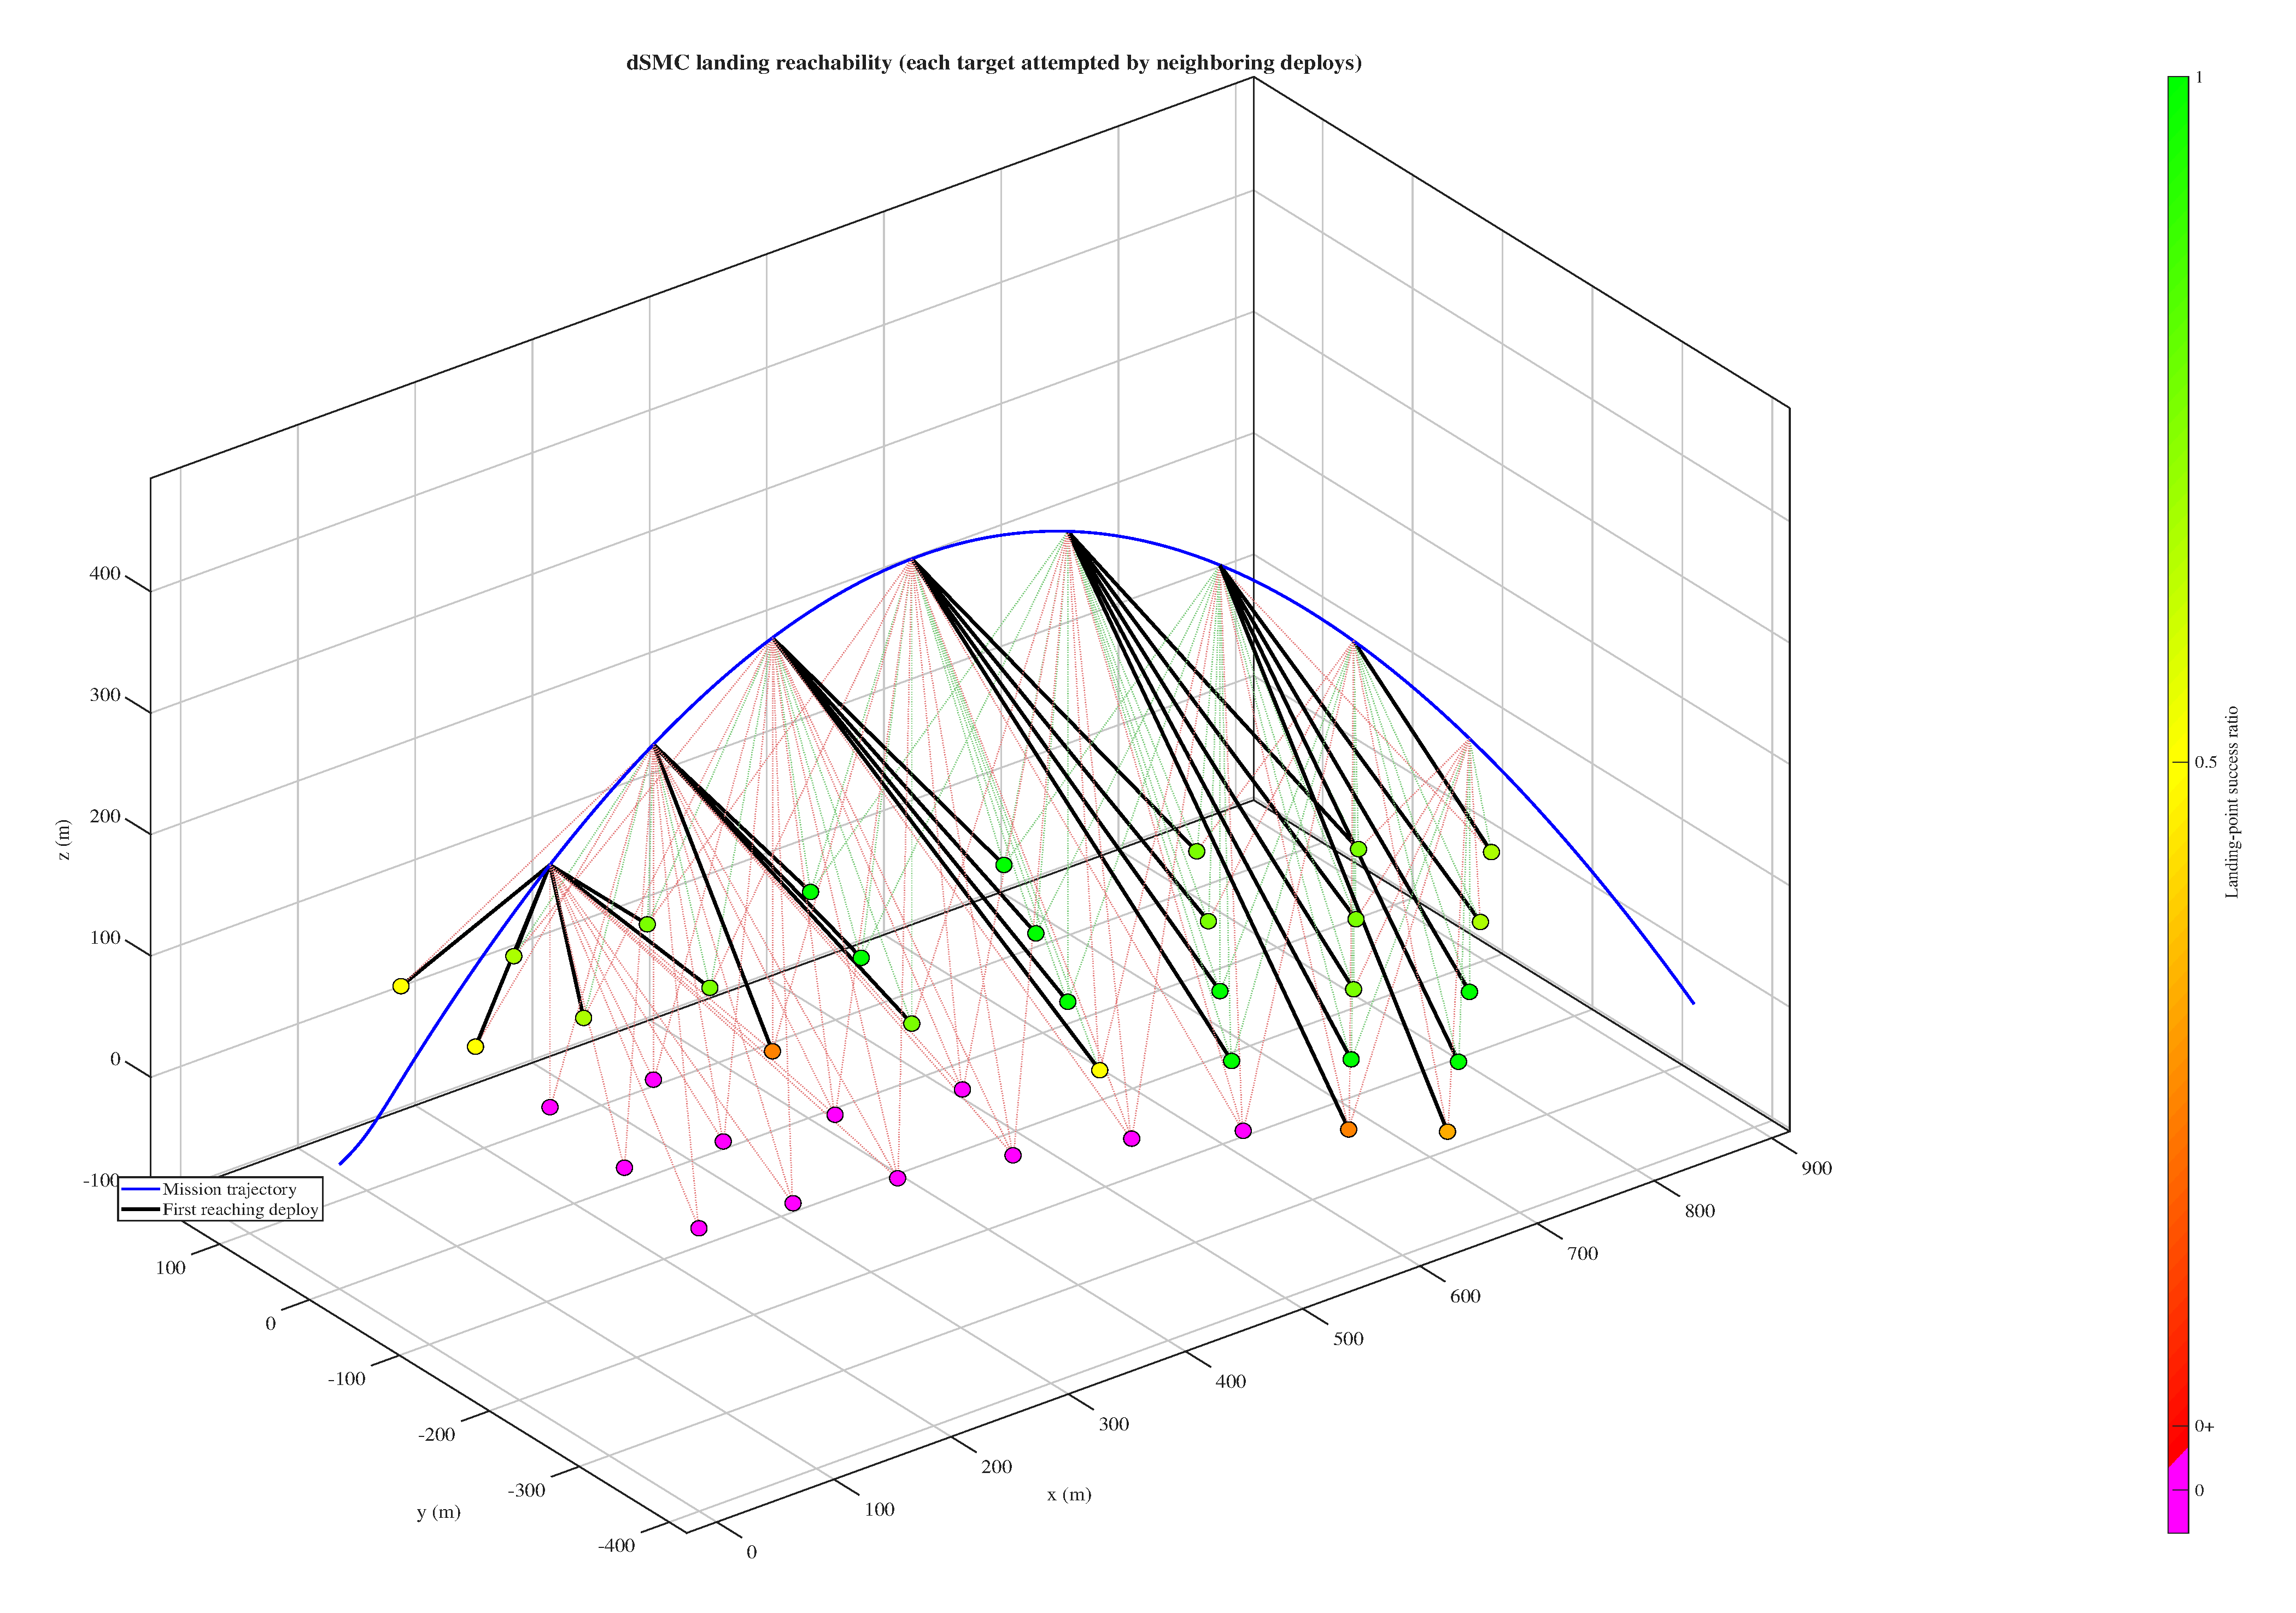
\includegraphics[width=0.8\linewidth]{figs/TO_04_landing_envelope_sat_on.eps}
\caption{Per-target landing reachability under saturation. Each landing target is attempted by neighboring deploys; markers are colored by the per-target success ratio, and black lines connect each target to its earliest reaching deploy.}
\label{fig:sat_landing_envelope_on}
\end{figure}

\begin{figure}[H]
\centering
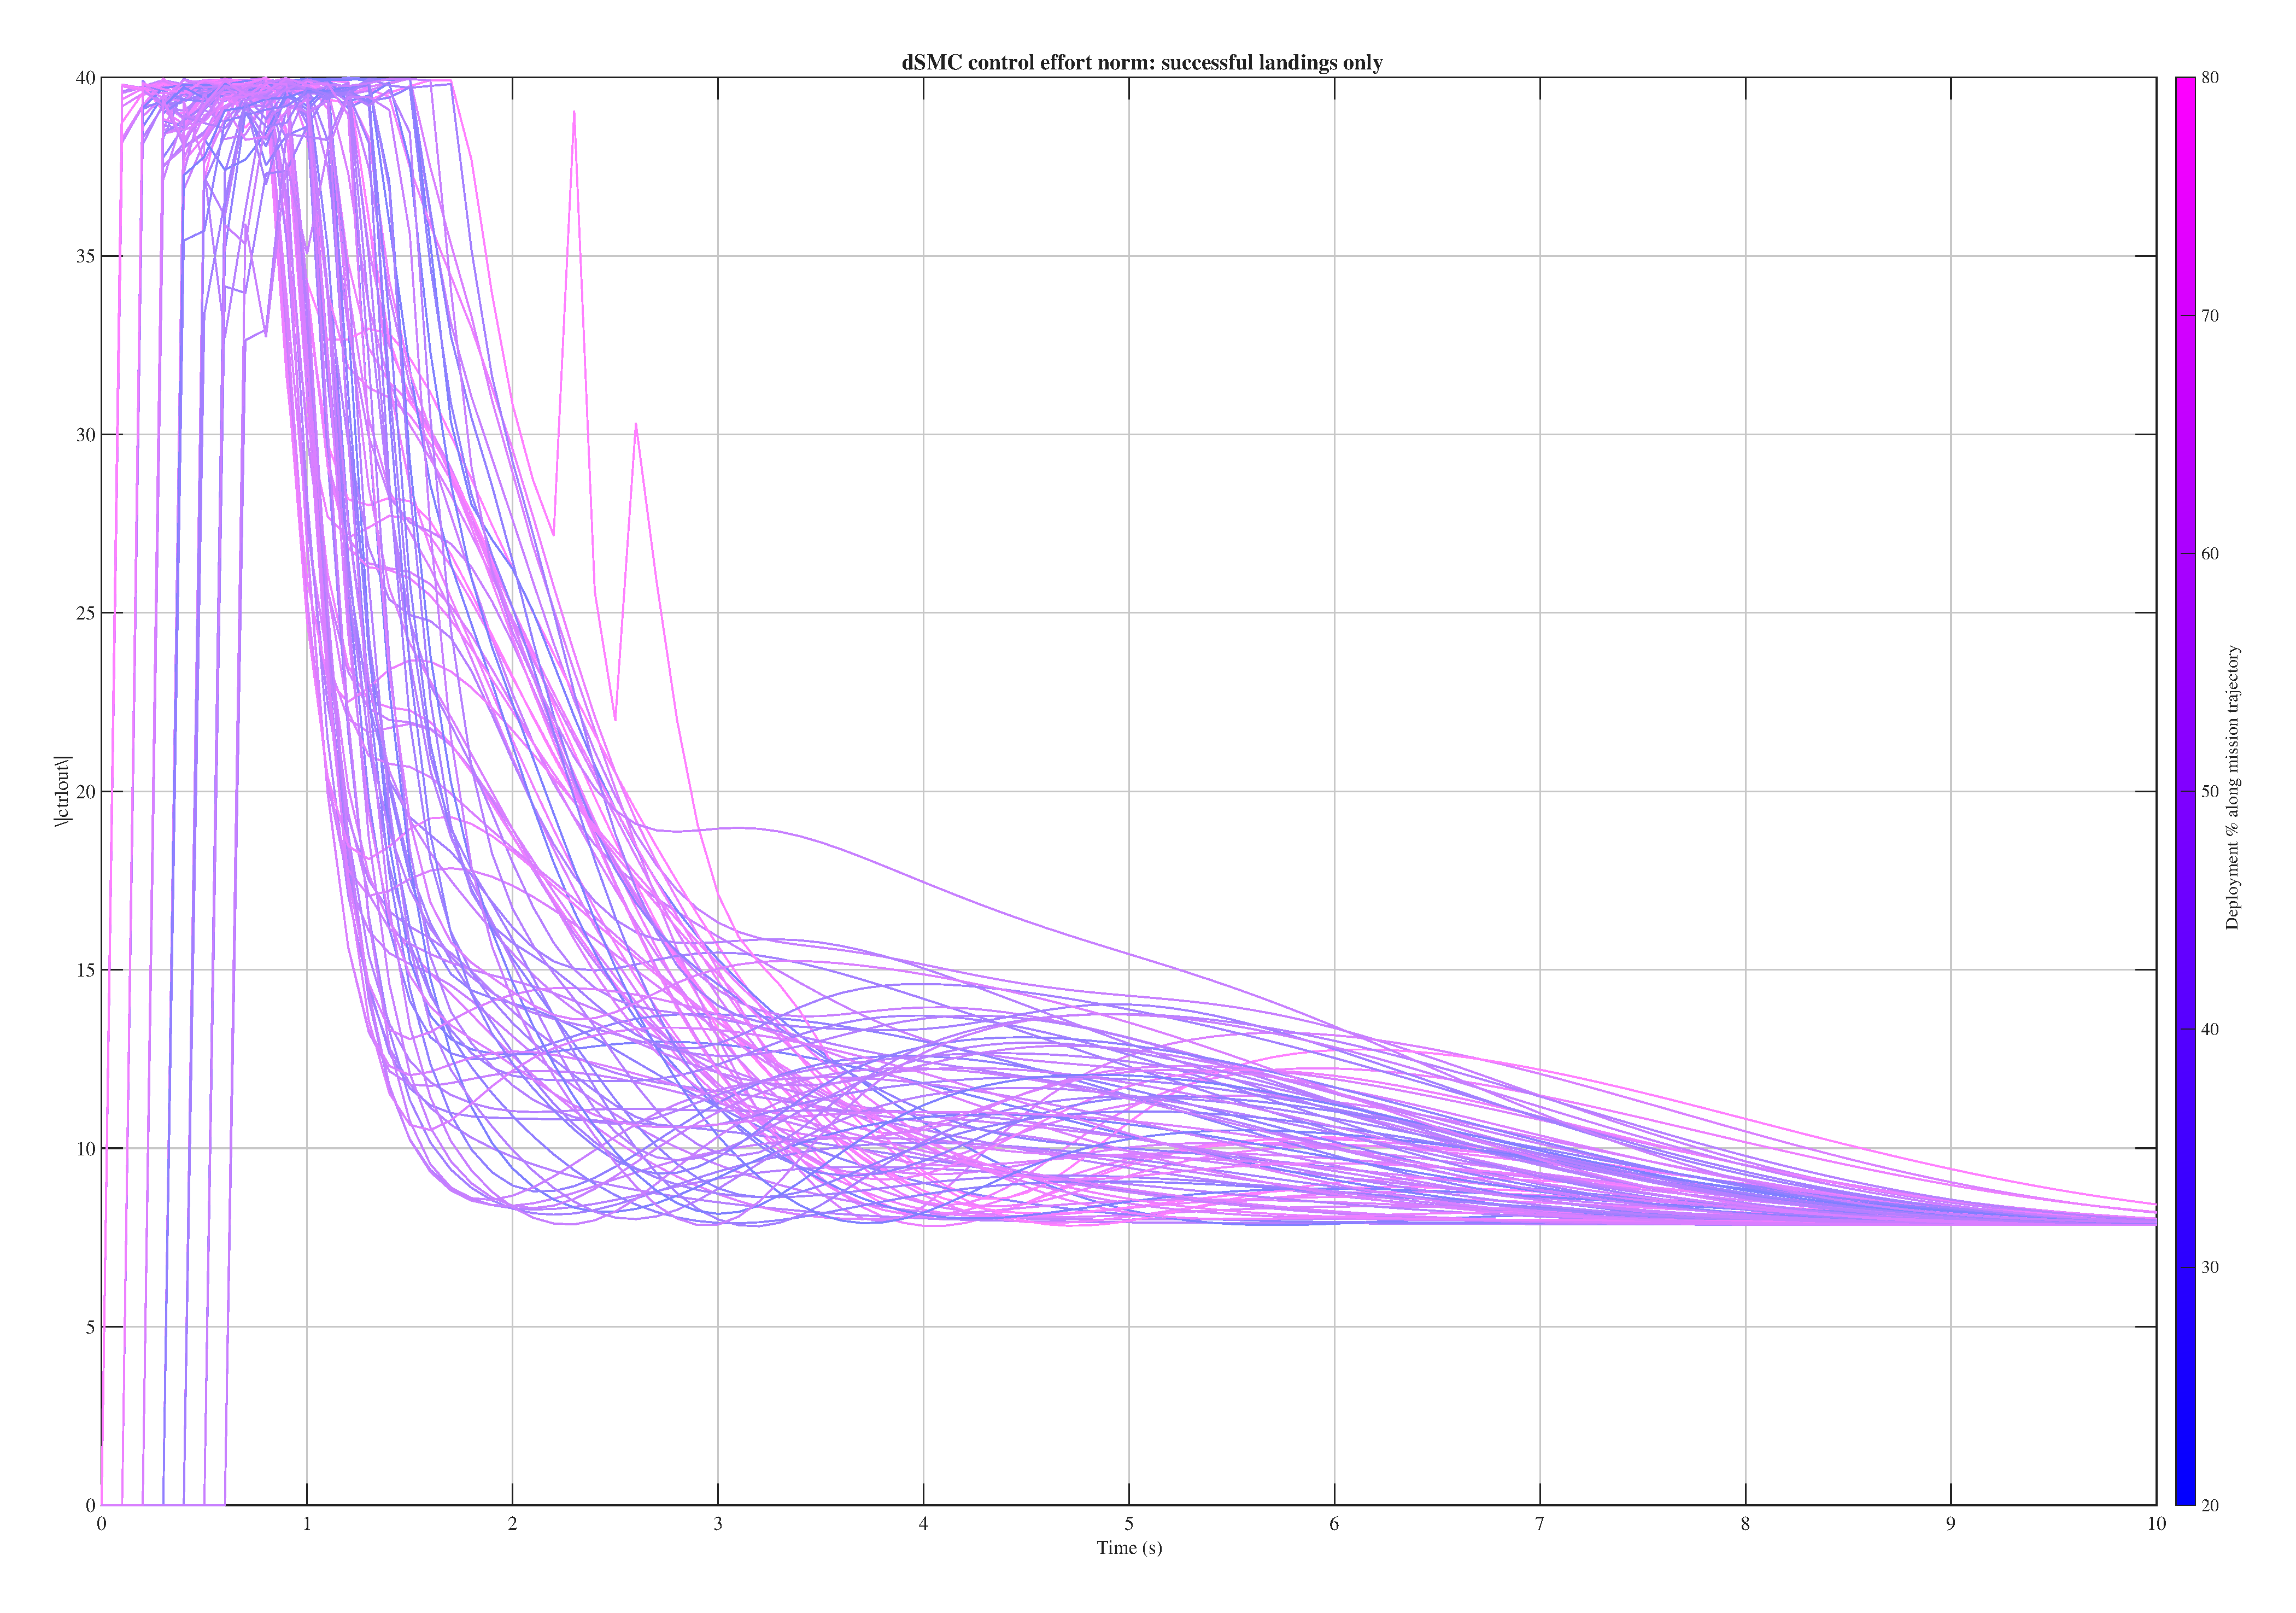
\includegraphics[width=0.8\linewidth]{figs/TO_06_control_norm_sat_on.eps}
\caption{Per-trial applied-command norm $|\bar u_k|$ during ballistic recovery with the saturation handler enabled, restricted to trials that achieved a successful landing. Traces are colored by deploy point along the mission trajectory.}
\label{fig:sat_control_norm_on}
\end{figure}

\begin{figure}[H]
\centering
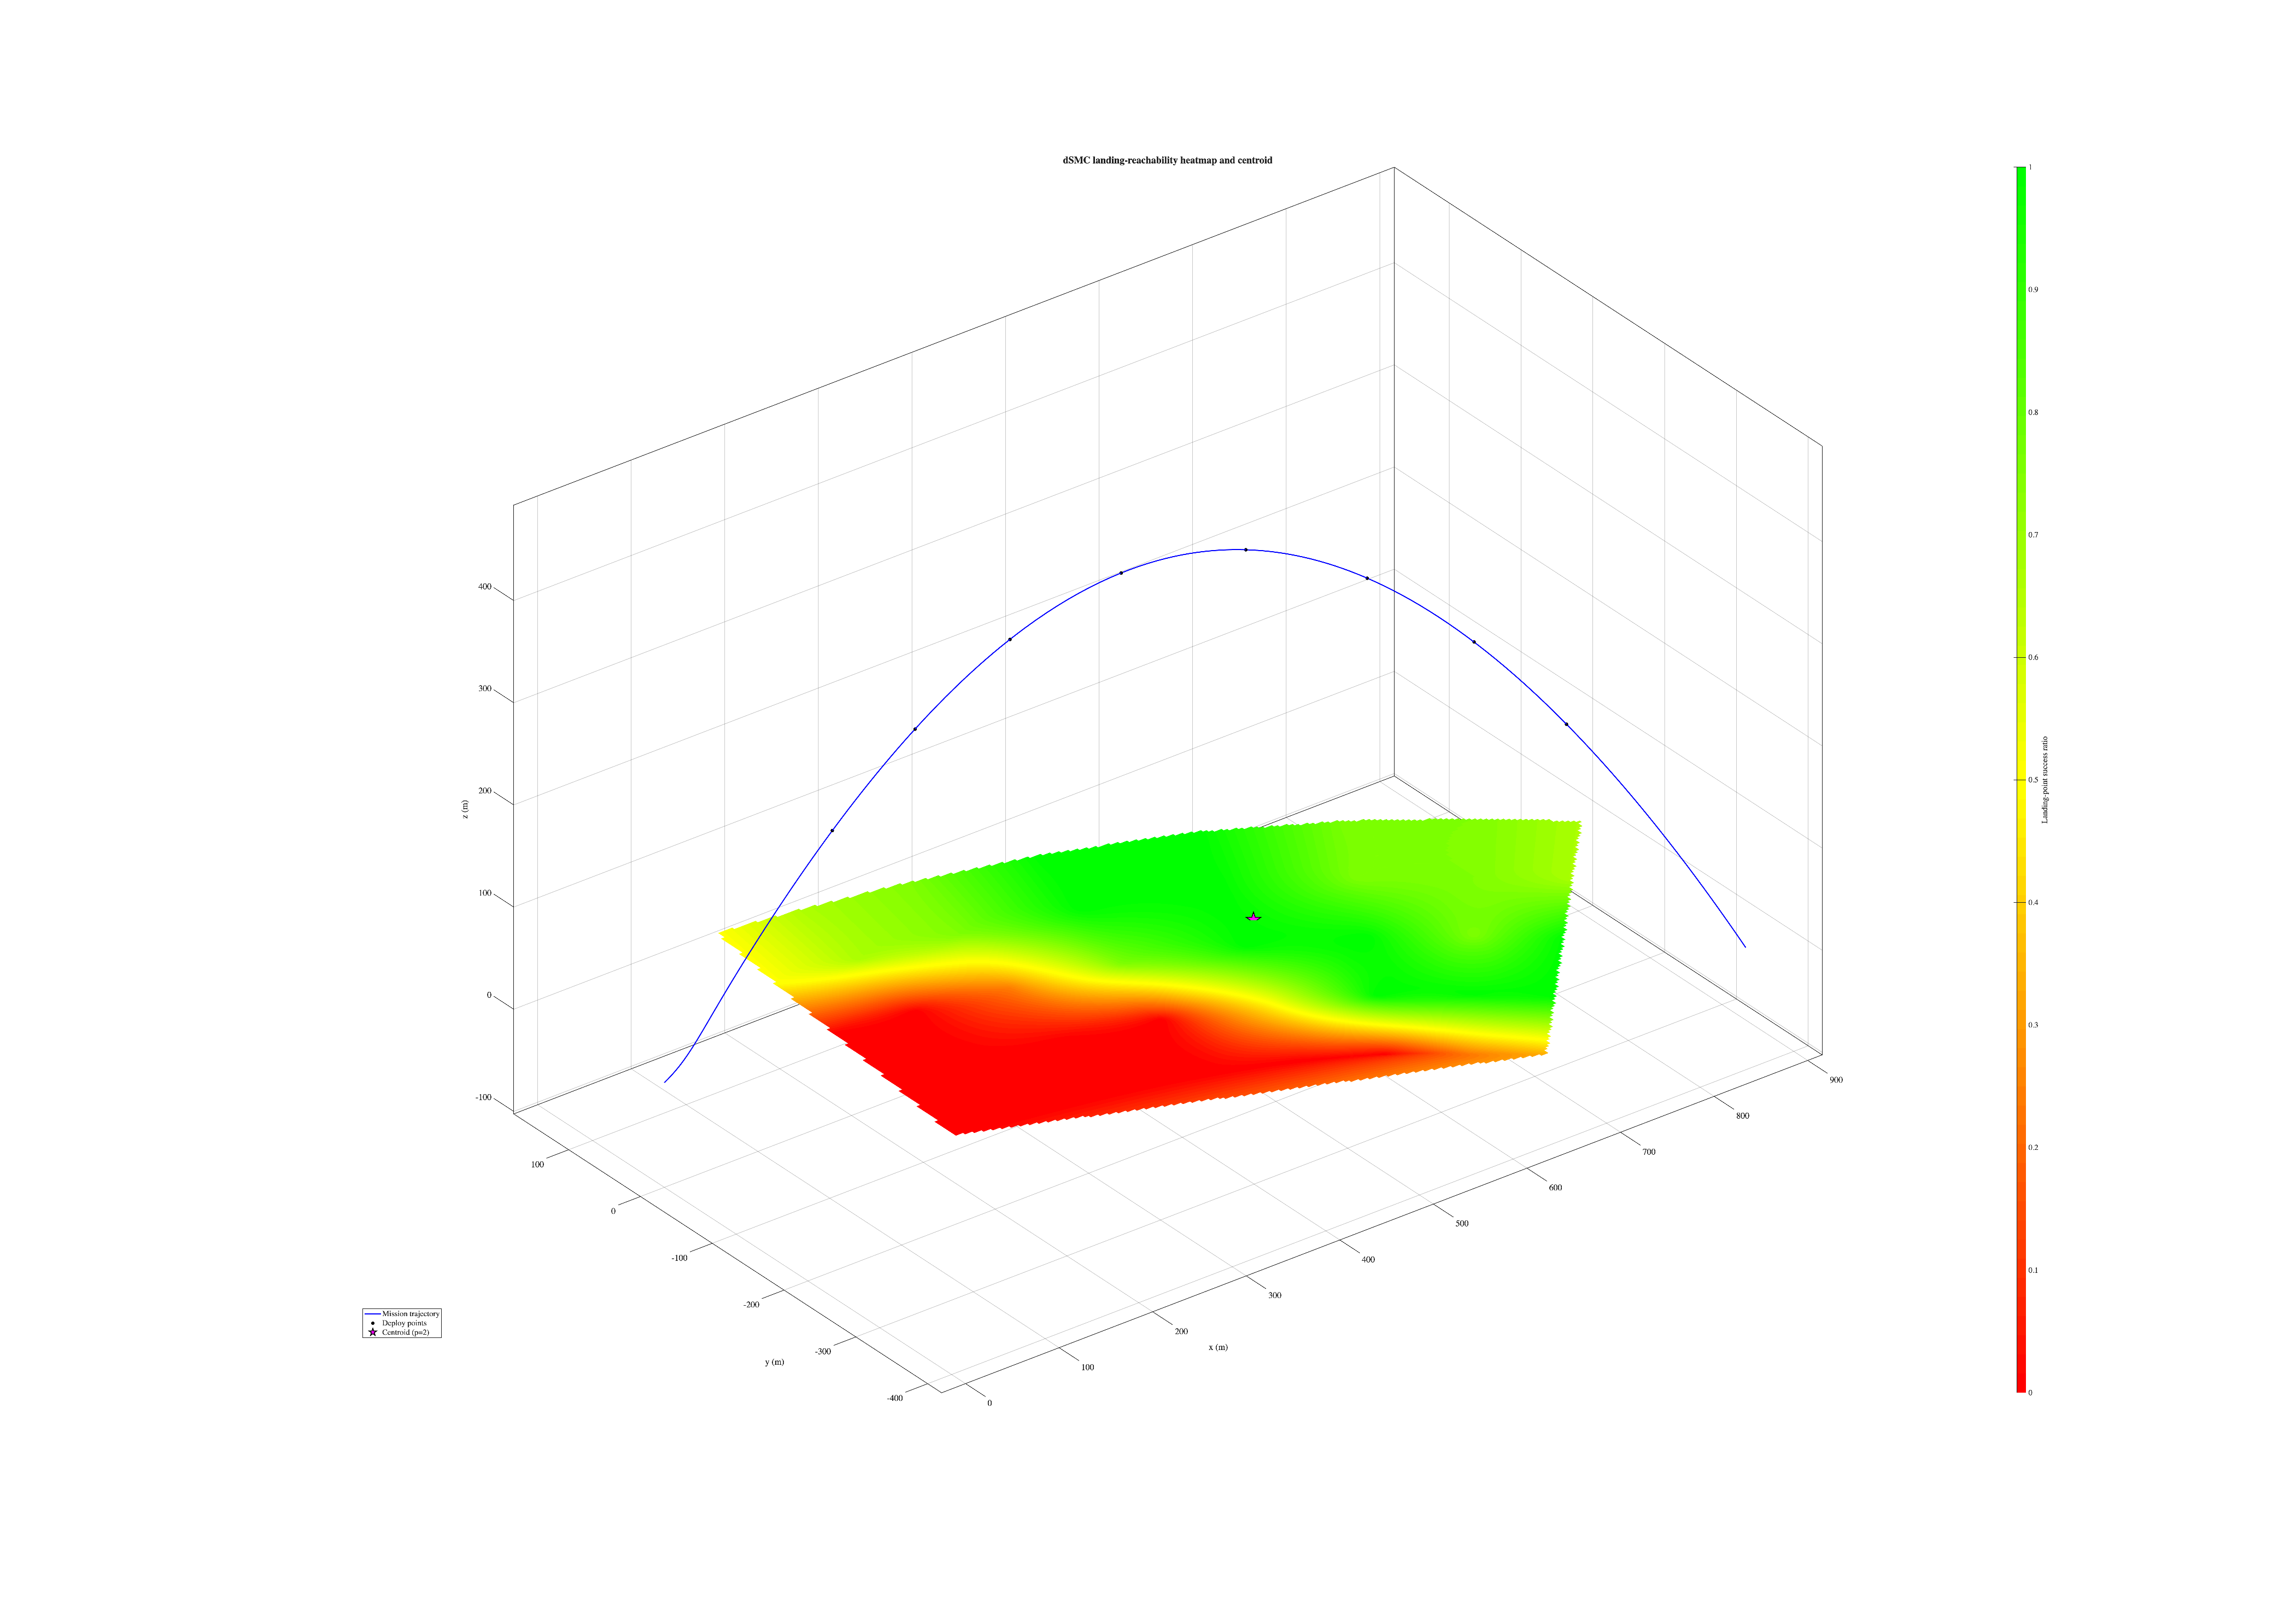
\includegraphics[width=0.8\linewidth]{figs/TO_07_landing_heatmap_sat_on.eps}
\caption{Landing-success ratio over the deploy~$\times$~cross-track sweep with the saturation handler enabled. The interpolated reachability surface is plotted beneath the ballistic mission trajectory, along with the power-weighted reachability centroid ($p = 2$, star).}
\label{fig:sat_landing_heatmap_on}
\end{figure}

\small
\begin{table}[t]
\centering
\caption{Landing-reachability statistics for the ballistic-recovery sweep with the saturation handler enabled versus the clipped baseline. Centroid uses the power-weighted estimator with $p = 2$.}
\label{tab:sat_cmp_summary}
\footnotesize
\setlength{\tabcolsep}{4pt}
\renewcommand{\arraystretch}{0.85}
\begin{tabular}{lcc}
\toprule
\textbf{Metric} & \textbf{Saturation} & \textbf{Control Clipping Only} \\
\midrule
Reachability fraction & $0.329$ & $0.079$ \\
Peak success ratio & $0.978$ & $0.292$ \\
Half-success radius (m) & $193.24$ & $156.19$ \\
Centroid $(x, y)$ (m) & $(453.04,\, -267.16)$ & $(430.53,\, -252.59)$ \\
\bottomrule
\end{tabular}
\end{table}
\normalsize

\section{Conclusions}
The dSMC recovers more of the ballistic-deployment envelope than the LQR, PID, or cSMC controllers, though no controller recovers every sampled state. Under motor-speed clipping the sweep reachability is $7.9\%$; the priority-weighted saturation handler raises it to $32.9\%$. This matters for launched-UAV operations because, given the smaller actuators of a launched UAV, control effort constraints can be severe. The COTS techniques (LQR and PID) and the continuous sliding mode controller do not stabilize the vehicle at most points along the trajectory - this is consistent with our intuition, as the COTS controllers assume linearity and the cSMC controller assumes continuity. For launched-drone operations, or for off-nominal initial conditions and aggressive flight in general, the dSMC formulation here beats the COTS controllers and, unlike cSMC, keeps its stability certificates under our discretized control plant.

\subsection{Future Work}
With an effective saturated controller and centroid generation logic in place, we want to additionally study the inverse problem of mapping from a desired centroid to the ballistic targeting variables (launch azimuth, elevation, velocity, exit spin, etc) required for a min-time landing, a max-likelihood landing, and a min-effort landing. Currently, we are examining numerical surrogate-based approaches to solving this, and have working prototypes in simulation. We plan to move to flight-test verification after, focusing on the ballistic case. Measuring real moments of inertia and drag parameters is the first step toward closing the sim-to-real gap. Inclement-weather operations will require a basic weather model. However, the stability certificates of both dSMC demonstrated on the ballistic envelope suggests that minor velocity and orientation perturbations won’t destabilize the controller.

%%%%%%%%%%%%%%%%%%%%%%%%%%%%%%%%%%%%%%%%%%%%%%%%%%%%%%%%%%%%%%%%%%%%%%%%%%%%%%%%
\section*{Acknowledgments}

The authors gratefully acknowledge the University of Texas at Austin for funding this preliminary work and appreciate the reviewers’ comments, with special thanks to members of the Clarke Research Group and Controls Group for Distributed and Uncertain Systems (CDUS).

\section*{Generative AI Statement}

The Anthropic Claude \cite{refs:claude} generative AI tool was used to improve the formatting and layout of the equations and tables, to reformat Microsoft Word equations to LaTeX formatting, to convert from MATLAB code to LaTeX equations, and to improve general syntax and grammar. The author assumes full responsibility for all results and derivations presented in this paper, and any errors which may be present therein.

%%%%%%%%%%%%%%%%%%%%%%%%%%%%%%%%%%%%%%%%%%%%%%%%%%%%%%%%%%%%%%%%%%%%%%%%%%%%%%%%

\bibliography{bibliography/aiaa_refs} % Entries are in the refs.bib file

\end{document}